\chapter{Sprint 4 : Exécution des Livraisons, Paiement \& Réclamations}

\section*{Introduction}
\addcontentsline{toc}{section}{Introduction}
Le Sprint~4 couvre l'exécution terrain des livraisons et le pilotage en temps réel. Le Chauffeur dispose sur son application mobile de toutes les fonctionnalités nécessaires pour démarrer une sortie, effectuer une checklist véhicule, valider les livraisons avec preuves numériques (signature, photos géolocalisées, scan d'articles) et traiter les paiements selon trois modes distincts : prépayé, chèque et traite. En cas d'incident, il peut signaler le problème directement depuis l'application. Le Planificateur suit la flotte en temps réel sur une carte GPS avec alertes automatiques de retard. Le REC rapproche les encaissements et traite les réclamations clients, escaladées automatiquement si non résolues dans les délais. Le Manager pilote l'ensemble de l'activité via des tableaux de bord KPI journaliers et des rapports exportables.

\clearpage

\section{Sprint Backlog}

\textbf{Objectif du sprint :} L'objectif est de couvrir l'exécution terrain : validation des livraisons avec preuves numériques, gestion des trois modes de paiement, suivi GPS en temps réel avec alertes de retard, traitement des réclamations avec escalade automatique et mode hors ligne mobile.

\definecolor{headerbg}{HTML}{d5f5e3}
\setlength{\arrayrulewidth}{1pt}

Les story points (SP) reflètent la complexité et l'effort de chaque tâche, estimés selon la suite de Fibonacci.

\begin{longtable}{|>{\raggedright\arraybackslash}p{4.2cm}|>{\raggedright\arraybackslash}p{4.8cm}|>{\raggedright\arraybackslash}p{4.5cm}|c|}
\hline
\rowcolor{headerbg}
\textbf{User Story} & \textbf{Tâche} & \textbf{Critères d'acceptation} & \textbf{\rotatebox{90}{SP}} \\
\hline
\endfirsthead
\hline
\rowcolor{headerbg}
\textbf{User Story} & \textbf{Tâche} & \textbf{Critères d'acceptation} & \textbf{\rotatebox{90}{SP}} \\
\hline
\endhead
\hline
\endfoot

%------ US-039 ------
\multirow{2}{=}{En tant que Chauffeur, je veux démarrer une livraison depuis l'application mobile et voir ses détails afin de préparer ma tournée.}
& Permettre au Chauffeur de consulter les détails d'une livraison (adresse, articles, créneau horaire) avant de la démarrer. & Les détails de la livraison s'affichent sur l'application mobile (adresse, liste d'articles, créneau horaire). & 2 \\
\cline{2-4}
& Mettre à jour automatiquement le statut de la commande au démarrage de la livraison et notifier le Planificateur. & Le statut passe à « En cours de livraison » ; le Planificateur est notifié en temps réel. & 1 \\
\hline

%------ US-040 ------
\multirow{2}{=}{En tant que Chauffeur, je veux confirmer une livraison avec la signature électronique du client depuis l'application mobile.}
& Permettre au Chauffeur de recueillir la signature du client sur écran tactile lors de la remise de commande. & La signature est capturée sur écran tactile, horodatée et transmise au système. & 3 \\
\cline{2-4}
& Faire passer la livraison au statut « Livrée » lors de la confirmation avec signature et notifier les parties concernées. & La livraison passe au statut « Livrée » ; la signature est rattachée à la livraison et consultable. & 2 \\
\hline

%------ US-041 ------
\multirow{2}{=}{En tant que Chauffeur, je veux prendre des photos géolocalisées comme preuve de livraison depuis l'application mobile.}
& Permettre au Chauffeur de prendre des photos géolocalisées lors de chaque livraison. & Les photos sont géolocalisées avec horodatage ; plusieurs photos peuvent être prises par livraison. & 2 \\
\cline{2-4}
& Rattacher les photos prises à la livraison concernée et les rendre consultables par le REC et le Manager. & Les photos sont consultables par le REC et le Manager dans l'historique de la livraison. & 1 \\
\hline

%------ US-042 ------
\multirow{2}{=}{En tant que Chauffeur, je veux valider les articles livrés depuis l'application mobile afin de confirmer la conformité de la commande.}
& Permettre au Chauffeur de valider les articles remis au client et détecter tout écart avec la commande prévue. & La validation des articles est réalisée ; tout écart entre les articles prévus et livrés génère une alerte. & 2 \\
\cline{2-4}
& Notifier le REC de tout écart constaté entre les articles prévus et effectivement livrés. & Un écart entre prévu et livré génère une alerte visible par le REC. & 1 \\
\hline

%------ US-043 ------
\multirow{2}{=}{En tant que Chauffeur, je veux signaler un problème de livraison depuis l'application mobile.}
& Permettre au Chauffeur de sélectionner le type de problème rencontré parmi une liste de motifs prédéfinis. & Le type de problème est sélectionné ; commentaire optionnel ; le statut de la livraison passe à « Échouée ». & 2 \\
\cline{2-4}
& Notifier automatiquement le Planificateur et le REC après le signalement d'un problème par le Chauffeur. & Le Planificateur et le REC reçoivent une notification immédiate avec les détails du problème. & 1 \\
\hline

%------ US-044 ------
\multirow{2}{=}{En tant que Planificateur, je veux suivre en temps réel la position des chauffeurs dans mon tableau de bord afin de superviser les tournées.}
& Afficher au Planificateur la position en temps réel de tous les chauffeurs actifs sur une carte. & La carte affiche tous les chauffeurs actifs ; les positions sont mises à jour régulièrement. & 3 \\
\cline{2-4}
& Afficher les alertes de retard directement sur la carte de suivi avec possibilité de filtrer par zone. & Les alertes de retard s'affichent automatiquement ; le filtrage par zone est disponible. & 2 \\
\hline

%------ US-045 ------
\multirow{2}{=}{En tant que Planificateur, je veux que le statut de la commande se mette à jour automatiquement à chaque action du Chauffeur afin de suivre l'avancement en temps réel.}
& Déclencher automatiquement les transitions de statut de la commande à partir des actions du Chauffeur sur l'application mobile. & Chaque action du Chauffeur déclenche la mise à jour du statut ; synchronisation en temps réel. & 2 \\
\cline{2-4}
& Notifier les parties prenantes concernées (REC, Client) à chaque changement de statut de la commande. & Les notifications sont envoyées aux bonnes parties prenantes à chaque transition de statut. & 1 \\
\hline

%------ US-046 ------
\multirow{2}{=}{En tant que REC, je veux générer un bordereau de livraison pour chaque tournée depuis mon application web.}
& Générer un document récapitulatif de tournée (bordereau) listant les livraisons, les articles et les clients concernés. & Le bordereau contient la liste des livraisons, les articles et les clients ; téléchargeable. & 2 \\
\cline{2-4}
& Permettre au REC de télécharger le bordereau depuis l'interface de gestion des tournées en un clic. & Le bordereau est généré et téléchargeable depuis l'interface en un clic. & 1 \\
\hline

%------ US-047 ------
\multirow{2}{=}{En tant que Chauffeur, je veux remplir un checklist de départ du véhicule sur l'application mobile avant le début de la journée.}
& Permettre au Chauffeur de remplir une liste de contrôles de départ avec prise de photos pour les anomalies constatées. & Le checklist est interactif ; les anomalies sont documentées avec photos. & 2 \\
\cline{2-4}
& Bloquer le démarrage de la tournée si les points critiques du checklist ne sont pas validés par le Chauffeur. & Le démarrage est bloqué si des points critiques ne sont pas validés ; une alerte est affichée. & 1 \\
\hline

%------ US-048 ------
\multirow{2}{=}{En tant que Client, je veux suivre ma livraison en temps réel sur une carte dans l'application mobile.}
& Afficher au Client la position du chauffeur sur une carte avec estimation de l'heure d'arrivée. & Le Client voit la position du chauffeur sur la carte ; l'estimation d'arrivée est mise à jour régulièrement. & 3 \\
\cline{2-4}
& Envoyer une notification au Client lorsque le chauffeur est à moins de 10 minutes de son adresse. & La notification est envoyée lorsque le chauffeur est à moins de 10 minutes de l'adresse. & 2 \\
\hline

%------ US-049 ------
\multirow{2}{=}{En tant que Planificateur, je veux que le système détecte automatiquement les retards et l'alerte afin de prendre des mesures correctives.}
& Détecter automatiquement un retard lorsqu'une livraison dépasse de plus de 15 minutes l'estimation initiale. & Une alerte est générée si le retard dépasse 15 minutes ; le statut de retard est affiché. & 2 \\
\cline{2-4}
& Notifier le Planificateur et le REC en cas de retard détecté avec les détails de la livraison concernée. & Le Planificateur et le REC reçoivent une alerte dans les 2 minutes suivant la détection. & 1 \\
\hline

%------ Mode 1 - Prépayé ------
\multirow{2}{=}{En tant que Planificateur, je veux voir le statut de paiement d'une commande afin d'autoriser ou bloquer la livraison.}
& Importer le statut de paiement depuis le système de gestion des commandes et l'afficher sur la fiche commande. & Le statut de paiement est importé avec la commande ; si prépayé, la livraison est autorisée automatiquement. & 2 \\
\cline{2-4}
& Afficher un indicateur « Prépayé » sur la commande visible par le Planificateur et le Chauffeur. & L'indicateur de paiement est visible sur l'interface web (Planificateur) et l'application mobile (Chauffeur). & 1 \\
\hline

%------ Mode 2 - Chèque ------
\multirow{2}{=}{En tant que Chauffeur, je veux photographier le chèque du client et l'envoyer au REC pour validation avant d'autoriser la livraison.}
& Permettre au Chauffeur de photographier le chèque et de l'envoyer en temps réel au REC pour traitement. & La photo est transmise et reçue par le REC en temps réel ; les informations du chèque sont extraites automatiquement. & 3 \\
\cline{2-4}
& Permettre au REC de valider le chèque et d'envoyer une autorisation de livraison au Chauffeur. & La validation par le REC déclenche une autorisation envoyée au Chauffeur ; en cas d'échec, le motif est communiqué. & 5 \\
\hline

%------ Mode 3 - Traite ------
\multirow{2}{=}{En tant que Chauffeur, je veux photographier une traite et l'envoyer au REC pour décision d'acceptation ou refus.}
& Permettre au Chauffeur de photographier la traite et de l'envoyer au REC pour décision. & La photo est transmise et reçue par le REC ; l'acceptation autorise la livraison ; le refus exige un motif. & 3 \\
\cline{2-4}
& Notifier le Chauffeur de la décision du REC (acceptation = livraison autorisée ; refus = retour marchandise). & Acceptation : livraison autorisée. Refus : motif enregistré et Chauffeur et Client notifiés. & 2 \\
\hline

%------ US-050 ------
\multirow{2}{=}{En tant que Manager, je veux consulter les indicateurs de livraison du jour dans mon tableau de bord.}
& Calculer et exposer au Manager les indicateurs de livraison du jour (livrées, en cours, en retard, échouées). & Le tableau de bord affiche les compteurs par statut mis à jour en temps réel. & 2 \\
\cline{2-4}
& Afficher au Manager les indicateurs de livraison du jour avec graphique d'évolution. & Les indicateurs s'actualisent automatiquement ; le taux de réussite et le graphique d'évolution sont affichés. & 1 \\
\hline

%------ US-063-067 ------
\multirow{2}{=}{En tant que Chauffeur, je veux consulter le récapitulatif de mes encaissements du jour depuis l'application mobile.}
& Calculer et exposer au Chauffeur le récapitulatif de ses encaissements du jour par mode de paiement et par montant. & Le récapitulatif affiche le total par mode (espèces, chèques, traites) et le nombre de transactions. & 2 \\
\cline{2-4}
& Afficher au Chauffeur l'écran d'encaissements avec liste détaillée et totaux par mode de paiement. & L'écran est accessible depuis l'application mobile ; les totaux sont corrects et mis à jour. & 1 \\
\hline

%------ US-068 ------
\multirow{2}{=}{En tant que REC, je veux rapprocher les encaissements avec les commandes livrées dans mon application web.}
& Permettre au REC de rapprocher les encaissements reçus avec les commandes livrées et de détecter les écarts. & L'association encaissement/commande fonctionne ; les écarts sont signalés et mis en évidence. & 3 \\
\cline{2-4}
& Afficher au REC la liste des encaissements avec indicateurs d'écarts et statut de rapprochement. & Le statut « Rapproché » est visible ; les écarts sont mis en évidence pour action corrective. & 2 \\
\hline

%------ US-105/107 ------
\multirow{2}{=}{En tant que Manager, je veux un tableau de bord stratégique avec export des rapports et visualisation des tendances.}
& Calculer les indicateurs stratégiques (taux de livraison, coût par kilomètre, satisfaction client, utilisation de la flotte) et les exposer au Manager. & Les indicateurs stratégiques sont disponibles avec comparaison par période. & 3 \\
\cline{2-4}
& Permettre au Manager d'exporter les rapports et de visualiser les tendances sur 30, 60 et 90 jours. & Les rapports sont exportables ; les graphiques de tendances sur 30/60/90 jours sont disponibles. & 2 \\
\hline


%------ US-105 ------
\multirow{2}{=}{En tant que Client, je veux soumettre une réclamation depuis l'application mobile afin d'obtenir un suivi.}
& Permettre au Client de soumettre une réclamation en précisant la catégorie, la description et des photos jointes. & La réclamation est créée avec catégorie, description et pièces jointes ; un numéro de suivi est généré. & 3 \\
\cline{2-4}
& Affecter automatiquement la réclamation au Responsable en charge du client concerné. & La réclamation est assignée au Responsable du client ; un numéro de ticket est communiqué au Client. & 2 \\
\hline

%------ US-106 ------
\multirow{2}{=}{En tant que Responsable des Engagements Clients, je veux voir la liste des réclamations et les traiter dans le respect du délai de service.}
& Mettre à disposition du REC la liste des réclamations avec filtres par statut, date et délai de service restant. & Les réclamations sont filtrables ; le délai de service restant (en jours) est affiché pour chaque réclamation. & 3 \\
\cline{2-4}
& Permettre au REC de prendre en charge, résoudre ou clôturer une réclamation avec notification au Client à chaque changement. & Le REC peut changer le statut ; le Client est notifié à chaque changement de statut. & 2 \\
\hline

%------ US-107 ------
\multirow{2}{=}{En tant que Client, je veux suivre le statut de ma réclamation depuis l'application mobile afin de rester informé de son traitement.}
& Permettre au Client de consulter l'état de sa réclamation avec l'historique des transitions de statut. & Le Client voit le statut en temps réel avec l'historique des transitions. & 2 \\
\cline{2-4}
& Notifier le Client à chaque changement de statut de sa réclamation. & Le Client est notifié en temps réel à chaque changement de statut. & 1 \\
\hline

%------ US-108/110 ------
\multirow{2}{=}{En tant que Manager, je veux des statistiques sur les réclamations et l'identification des causes récurrentes dans mon tableau de bord.}
& Calculer les indicateurs de réclamations (volume, délai moyen de traitement, taux de récurrence, causes principales) et les exposer au Manager. & Les statistiques incluent : nombre par catégorie, délai moyen, taux de récurrence. & 3 \\
\cline{2-4}
& Afficher les causes les plus fréquentes de réclamations dans une vue comparative dans le tableau de bord Manager. & Les principales causes de réclamations s'affichent par ordre de fréquence décroissante. & 2 \\
\hline

%------ US-109 ------
\multirow{2}{=}{En tant que Responsable des Engagements Clients, je veux que les réclamations non traitées soient escaladées automatiquement après 48 heures afin de respecter les délais de réponse.}
& Déclencher automatiquement l'escalade d'une réclamation non traitée après 48 heures avec notification au Manager. & L'escalade est déclenchée après 48 heures ; le Manager est notifié avec les détails de la réclamation. & 2 \\
\cline{2-4}
& Mettre en évidence les réclamations escaladées dans la liste du REC avec un indicateur d'urgence visible. & Les réclamations escaladées affichent un indicateur d'urgence dans la liste. & 1 \\
\hline

%------ US-119/120 ------
\multirow{2}{=}{En tant que Manager, je veux personnaliser mon tableau de bord avec des widgets configurables et exporter les rapports.}
& Permettre au Manager de réorganiser les widgets de son tableau de bord et de sauvegarder sa configuration. & Les widgets sont déplaçables ; la configuration est sauvegardée par profil utilisateur. & 3 \\
\cline{2-4}
& Permettre au Manager d'exporter les rapports du tableau de bord dans des formats standards. & Les rapports sont exportables depuis tous les tableaux de bord ; la mise en page est professionnelle. & 2 \\
\hline

%------ US-140/141/142 ------
\multirow{2}{=}{En tant que Chauffeur, je veux utiliser l'application mobile en mode hors ligne et que mes actions se synchronisent automatiquement au retour du réseau.}
& Permettre au Chauffeur d'utiliser les fonctionnalités essentielles de l'application sans connexion réseau, avec mise en file d'attente des actions. & Les données essentielles sont disponibles hors ligne ; les actions sont mises en file d'attente et exécutées au retour du réseau. & 5 \\
\cline{2-4}
& Synchroniser automatiquement les données au retour du réseau avec gestion des conflits éventuels et indicateur de statut de connexion. & La synchronisation démarre automatiquement ; les conflits critiques sont signalés ; un indicateur de connexion est visible. & 3 \\
\hline

%------ US-121/122/123 ------
\multirow{2}{=}{En tant que Manager, je veux voir les tendances sur 30, 60 et 90 jours et un tableau de bord de performance des chauffeurs avec rapports automatisés.}
& Calculer les indicateurs historiques sur 30, 60 et 90 jours avec détection des anomalies et les présenter au Manager. & Les graphiques affichent les tendances ; les anomalies sont détectées et mises en évidence. & 3 \\
\cline{2-4}
& Envoyer automatiquement des rapports récapitulatifs hebdomadaires aux destinataires configurés. & Les rapports hebdomadaires sont envoyés automatiquement aux destinataires configurés. & 2 \\
\hline

\caption{Sprint Backlog du Sprint 4 --- Exécution des Livraisons, Paiement \& Réclamations}
\end{longtable}
\setlength{\arrayrulewidth}{0.4pt}


% =============================================================
\section{Conception}
% =============================================================

\subsection{Diagramme de cas d'utilisation}

\begin{figure}[H]
\centering
\IfFileExists{img/diagrammes/sprint_4_usecase_p1.png}{%
  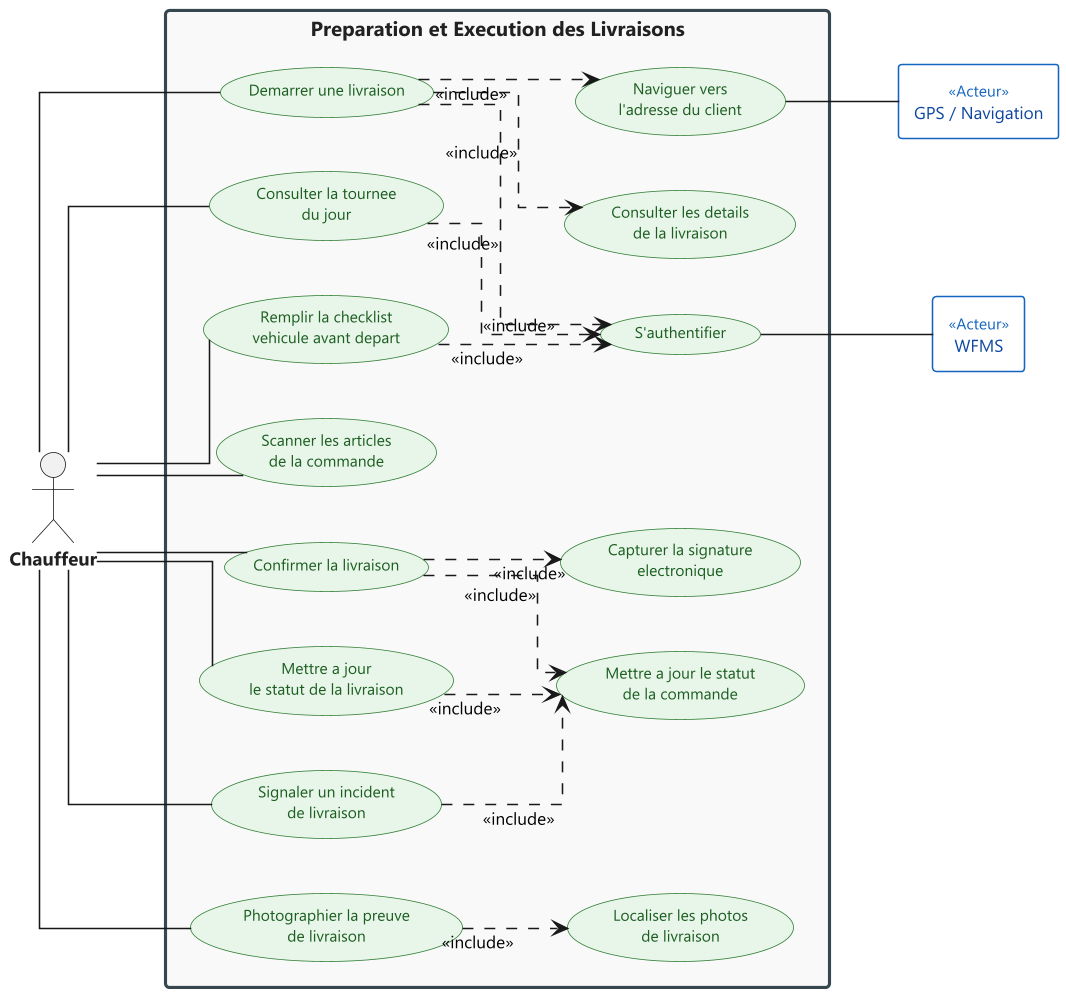
\includegraphics[width=0.9\textwidth, height=0.85\textheight, keepaspectratio]{img/diagrammes/sprint_4_usecase_p1}%
}{%
  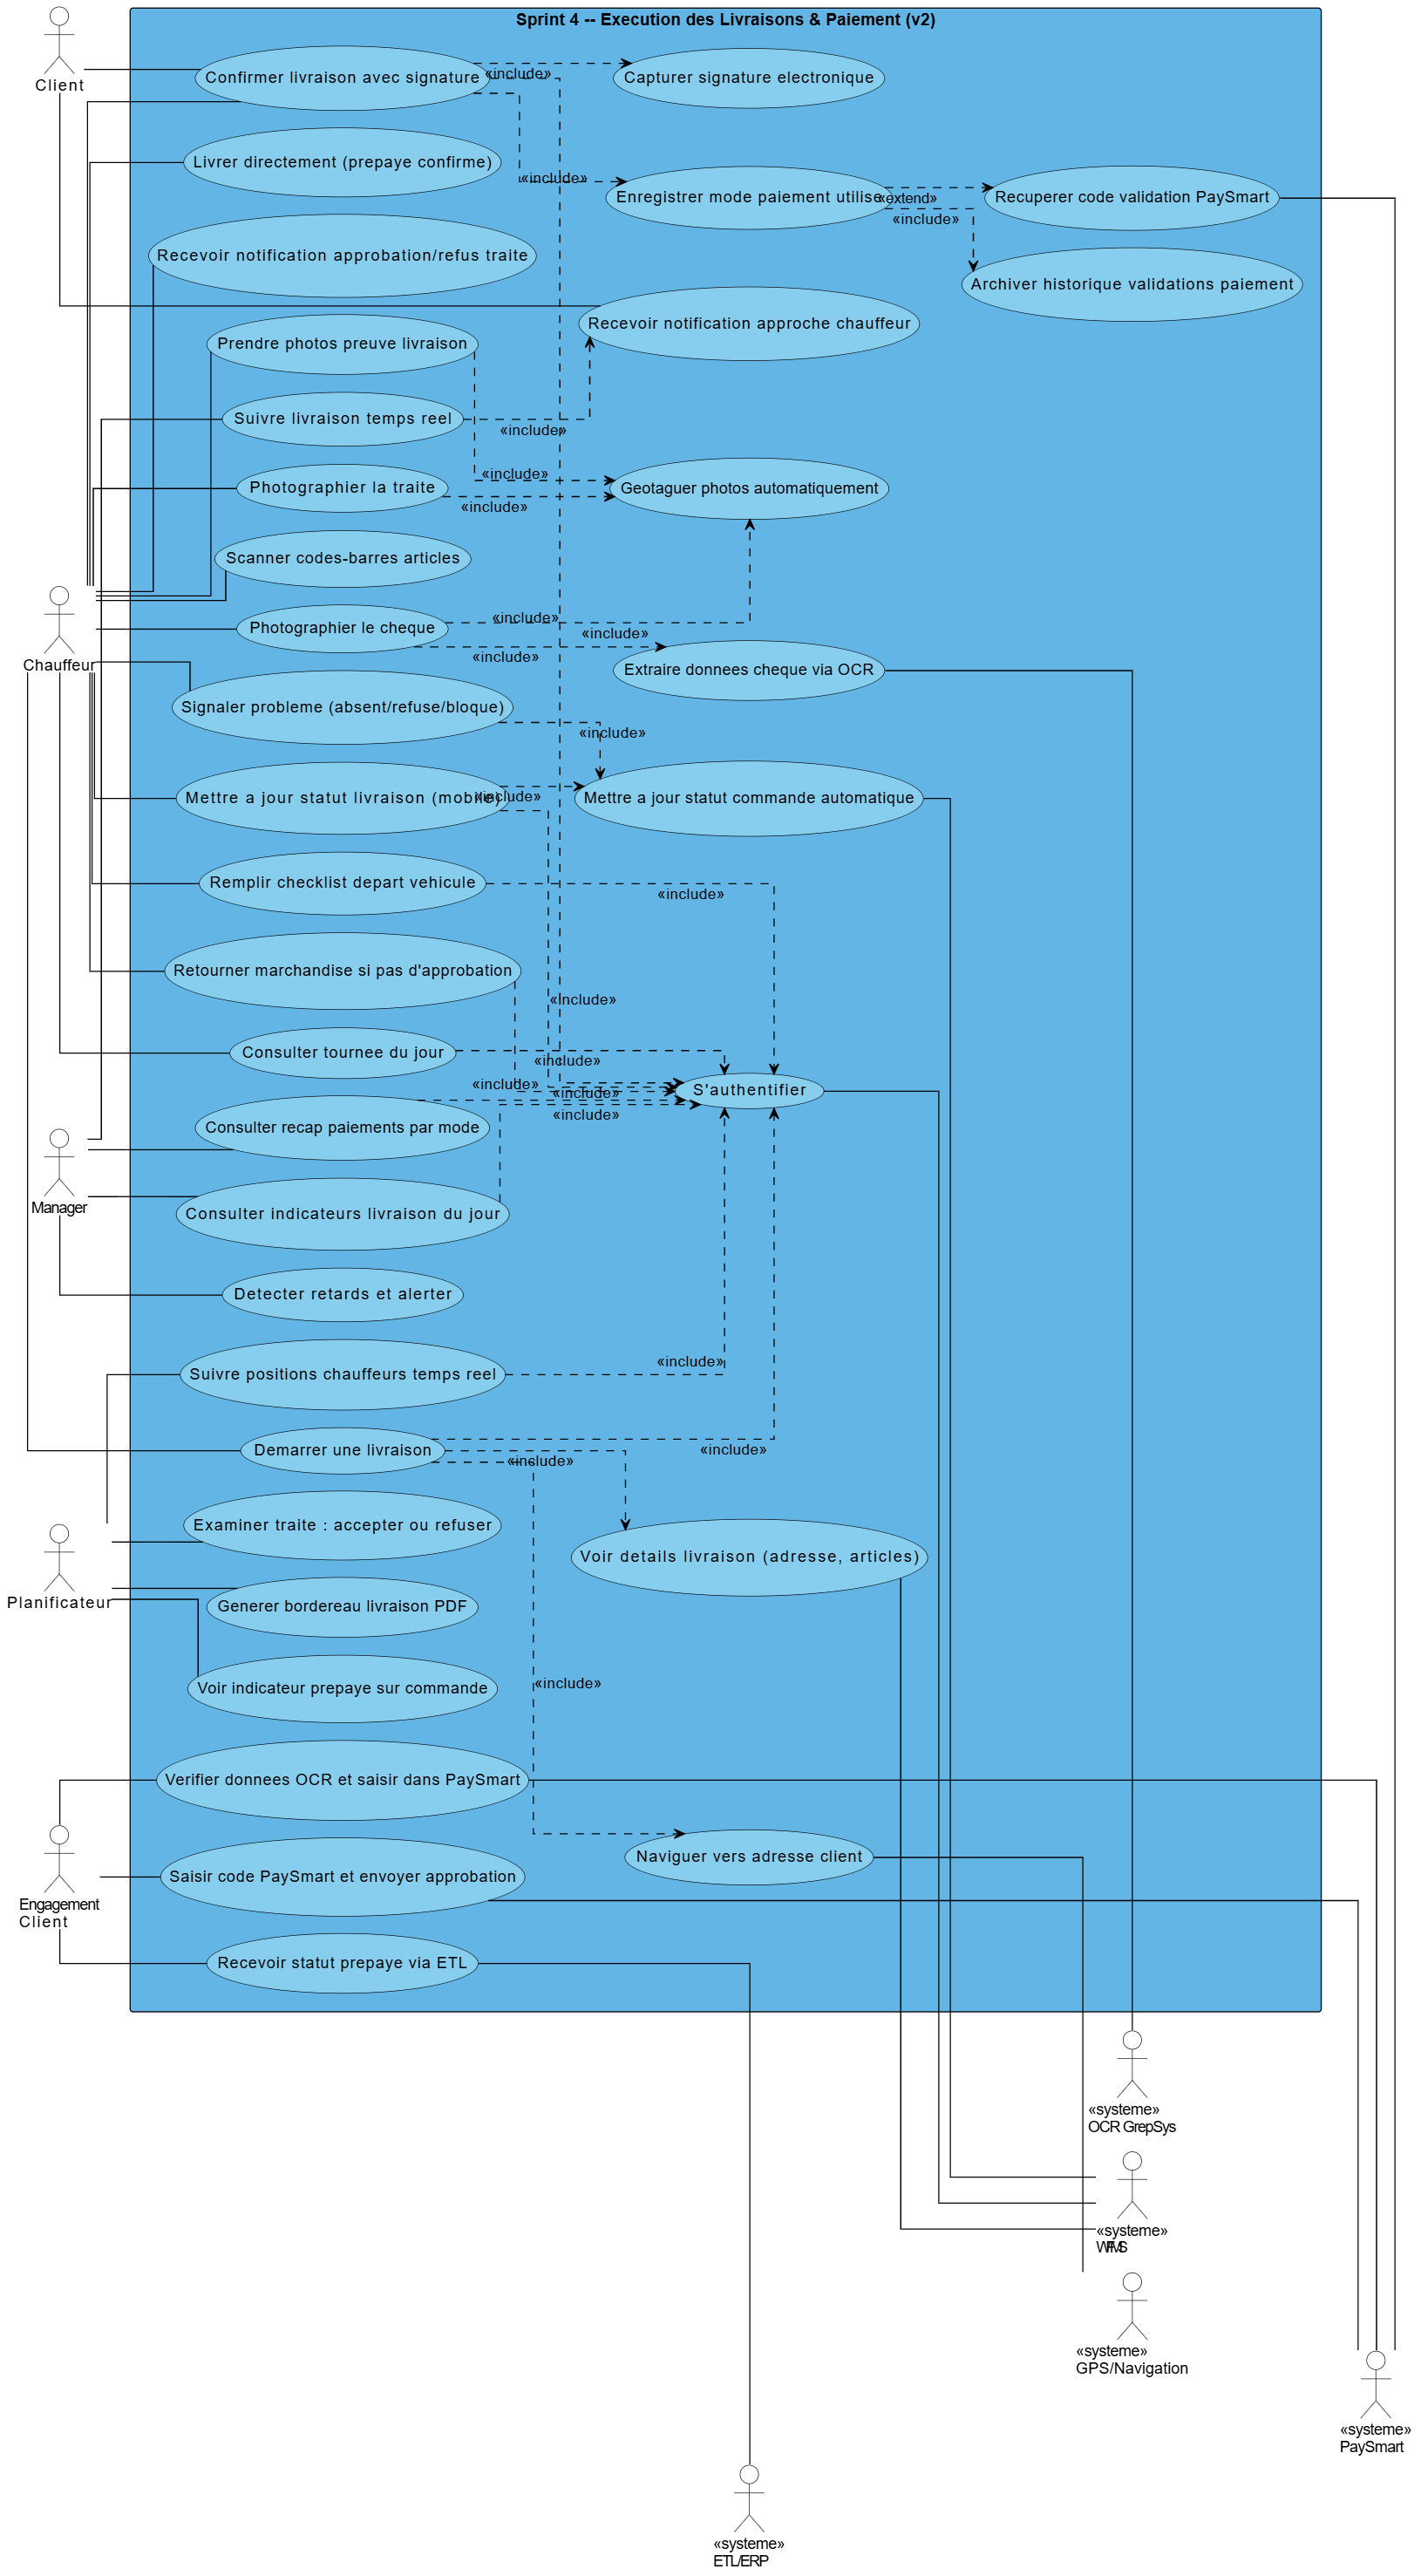
\includegraphics[width=0.9\textwidth, height=0.85\textheight, keepaspectratio]{img/diagrammes/sprint_4_usecase}%
}
\caption{Diagramme de cas d'utilisation du Sprint~4 --- Partie~1}
\label{fig:cas-utilisation-sp4-p1}
\end{figure}

\begin{figure}[H]
\centering
\IfFileExists{img/diagrammes/sprint_4_usecase_p2.png}{%
  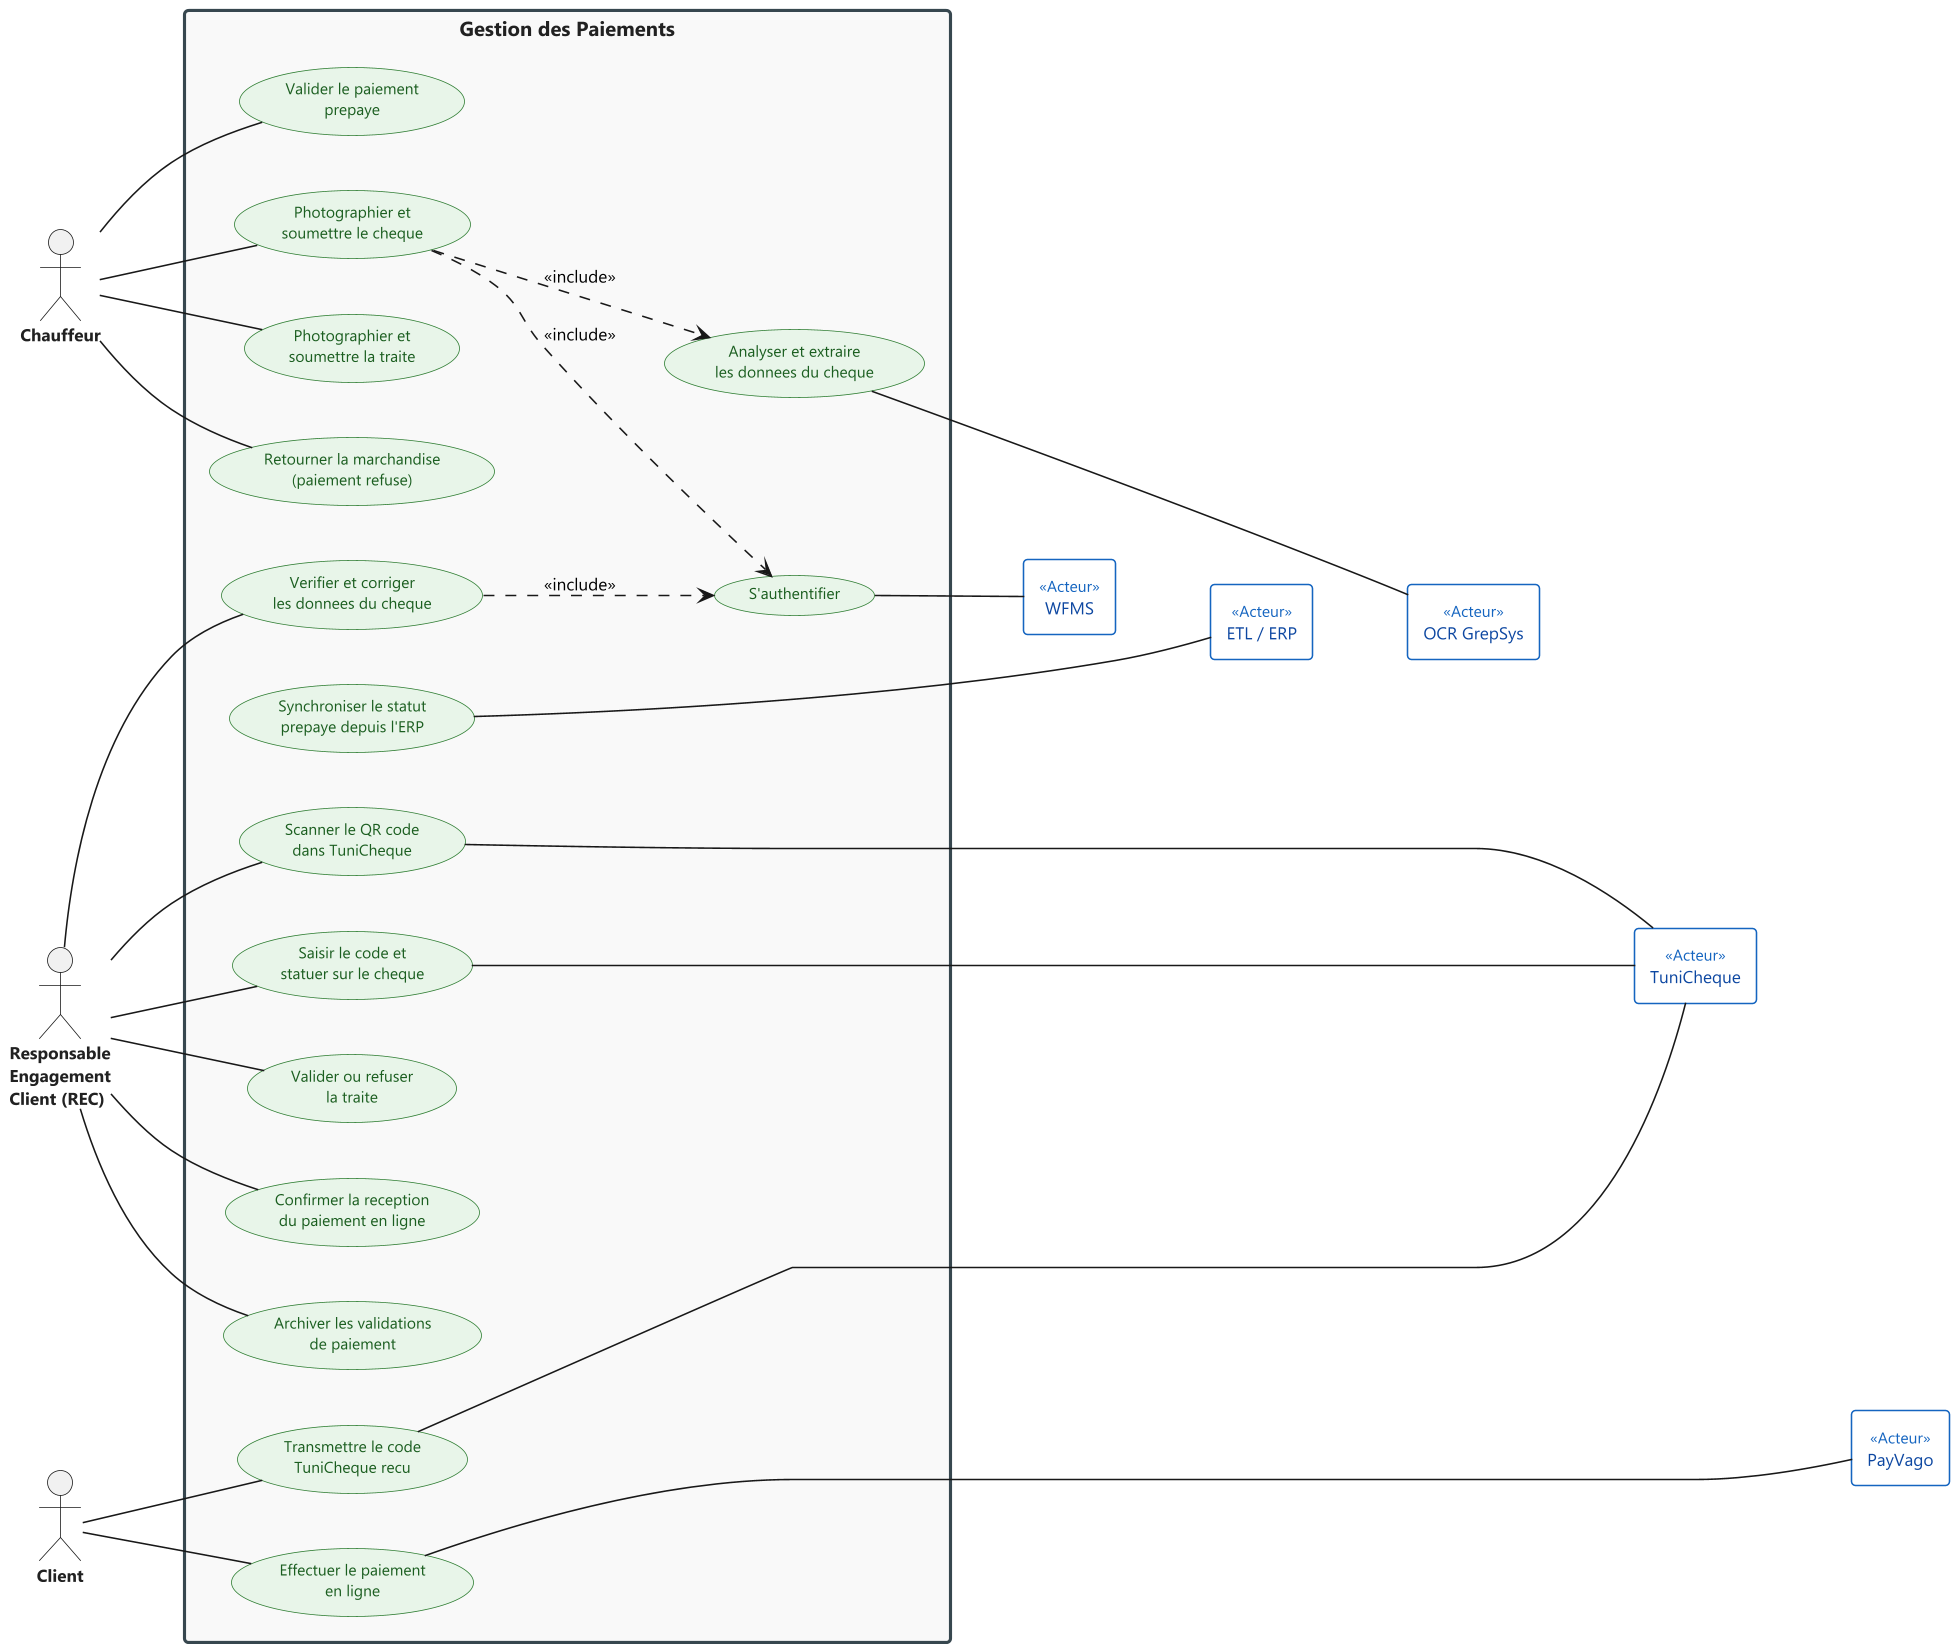
\includegraphics[width=0.9\textwidth, height=0.85\textheight, keepaspectratio]{img/diagrammes/sprint_4_usecase_p2}%
}{%
  \fbox{\parbox{0.9\linewidth}{\centering\vspace{4cm}\textit{[img/diagrammes/sprint\_4\_usecase\_p2.png]}\vspace{4cm}}}%
}
\caption{Diagramme de cas d'utilisation du Sprint~4 --- Partie~2}
\label{fig:cas-utilisation-sp4-p2}
\end{figure}

\begin{figure}[H]
\centering
\IfFileExists{img/diagrammes/sprint_4_usecase_p3.png}{%
  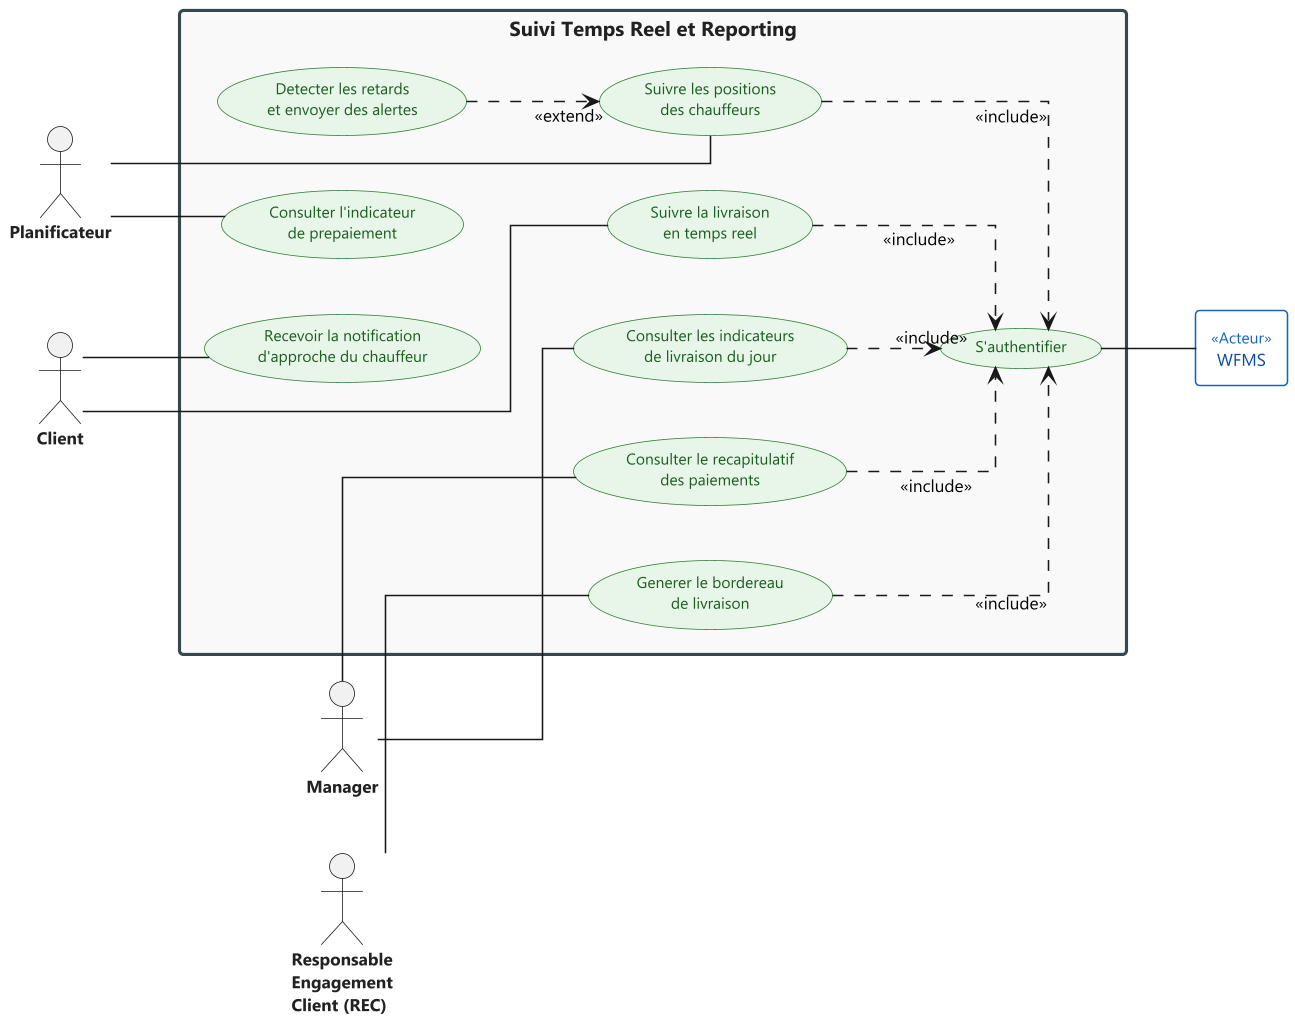
\includegraphics[width=0.9\textwidth, height=0.85\textheight, keepaspectratio]{img/diagrammes/sprint_4_usecase_p3}%
}{%
  \fbox{\parbox{0.9\linewidth}{\centering\vspace{4cm}\textit{[img/diagrammes/sprint\_4\_usecase\_p3.png]}\vspace{4cm}}}%
}
\caption{Diagramme de cas d'utilisation du Sprint~4 --- Partie~3}
\label{fig:cas-utilisation-sp4-p3}
\end{figure}

\subsection{Description textuelle}

\captionsetup[longtable]{justification=centering}
\setlength{\arrayrulewidth}{1pt}
\begin{longtable}{|p{4cm}|p{11cm}|}
\hline
\rowcolor{headerbg}
\textbf{Élément} & \textbf{Description} \\
\hline
\textbf{Titre} & Confirmer une livraison \\
\hline
\textbf{Acteurs} & Chauffeur, Responsable des Engagements Clients (REC), Planificateur \\
\hline
\textbf{Objectif} & Permettre au Chauffeur de valider la remise de la marchandise avec preuves numériques depuis l'application mobile, et au Planificateur/Manager de suivre l'exécution en temps réel depuis l'interface web. \\
\hline
\textbf{Précondition} & La livraison est au statut EN\_COURS. Le paiement est validé (ou le mode est prépayé). Le Chauffeur est connecté à l'app mobile. \\
\hline
\textbf{Postcondition} & La livraison passe au statut LIVRÉE. La preuve est archivée (chiffrement AES-256, 5 ans). Le client et le REC sont notifiés. \\
\hline
\textbf{Scénario nominal} &
\begin{enumerate}[start=1, label=\arabic*.]
    \item Le Chauffeur ouvre la livraison depuis l'app mobile et clique sur « Confirmer ».
    \item Le client signe sur l'écran tactile ; la signature est encodée en base64.
    \item Le Chauffeur prend des photos géolocalisées horodatées de la marchandise livrée.
    \item Le Chauffeur valide les articles remis et détecte tout écart avec la commande.
    \item Le système enregistre la preuve et passe la livraison au statut LIVRÉE.
    \item Le Planificateur voit la mise à jour en temps réel sur la carte GPS et le tableau de bord KPI.
    \item Le REC génère le bordereau de livraison depuis l'interface web.
\end{enumerate} \\
\hline
\textbf{Scénario alternatif} &
\begin{enumerate}[start=1, label=\arabic*.]
    \item Client absent : le Chauffeur sélectionne le motif « Client absent » ; statut passe à ÉCHOUÉE.
    \item Article non conforme : une alerte est générée et envoyée au REC.
    \item Mode de paiement non validé : la confirmation est bloquée jusqu'à l'approbation REC.
    \item Livraison échouée non traitée : le Planificateur la reprogramme en priorité le lendemain.
\end{enumerate} \\
\hline
\caption{Description textuelle --- Confirmer une livraison (Sprint 4)}
\end{longtable}
\setlength{\arrayrulewidth}{0.4pt}

\subsection{Diagramme de classes}

\newpage
\thispagestyle{empty}
\begin{landscape}
\begin{figure}[H]
\centering
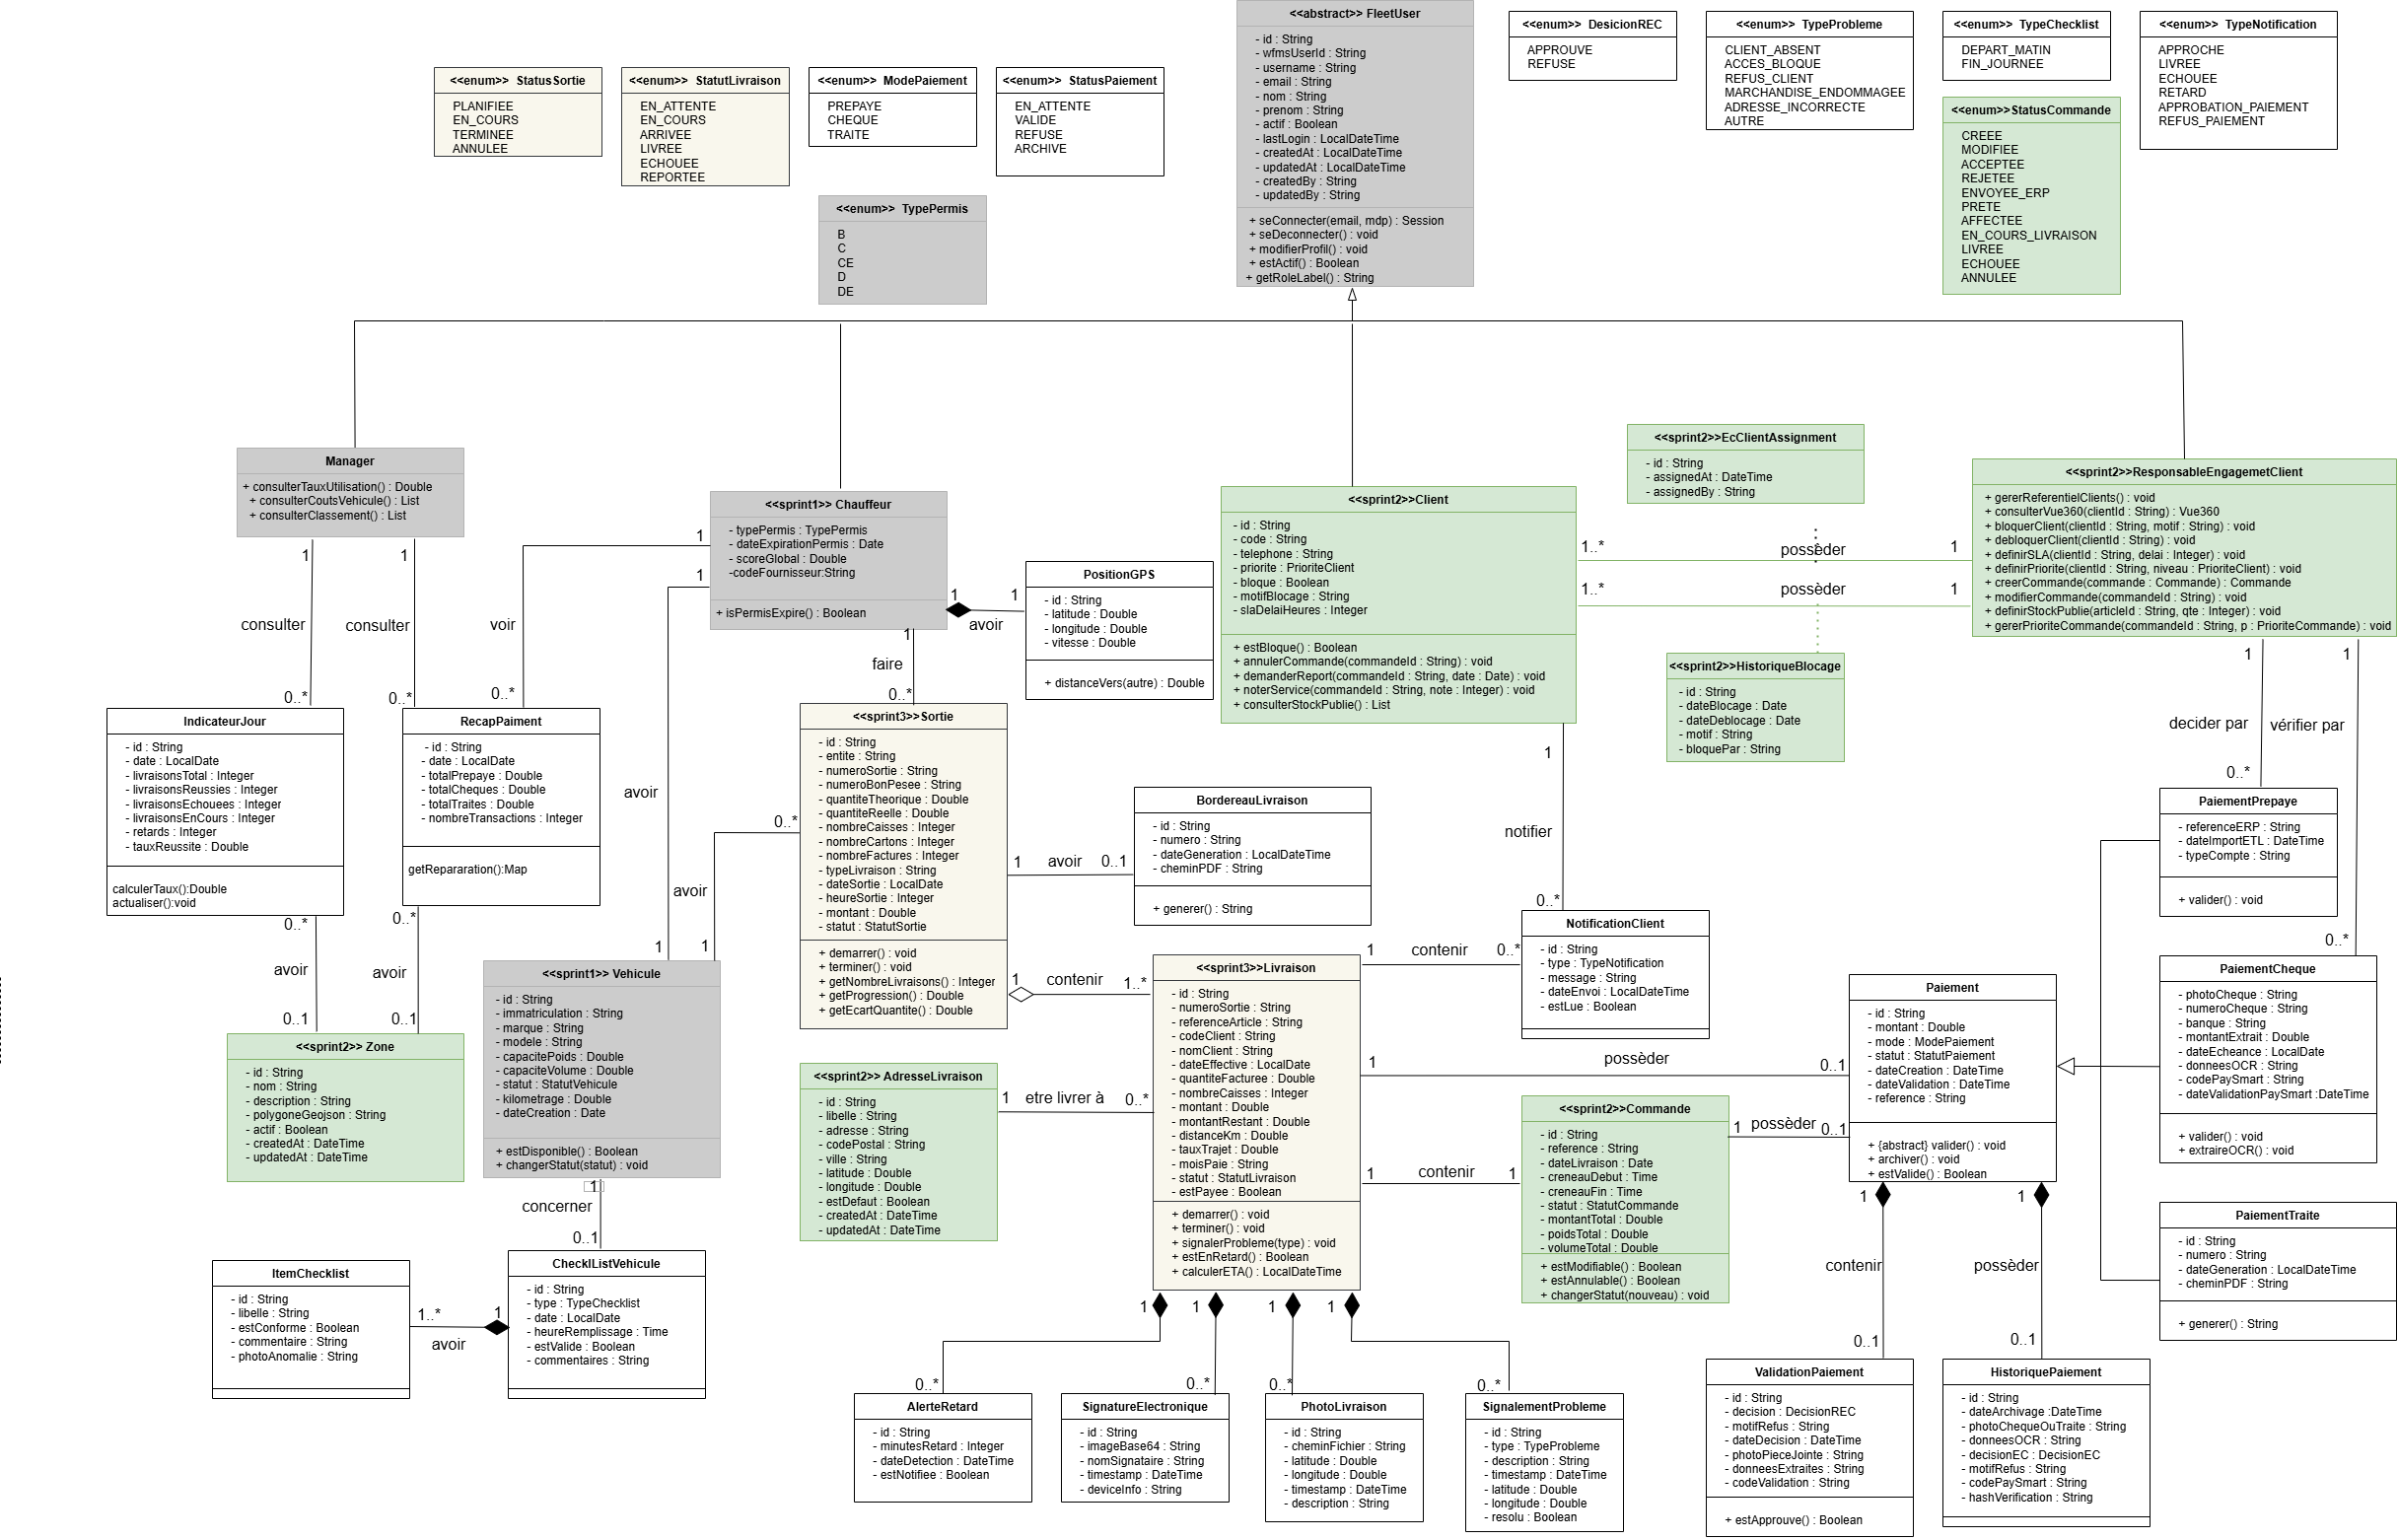
\includegraphics[width=\linewidth, height=0.95\textheight, keepaspectratio]{img/diagrammes/sprint_4_classes}
\caption{Diagramme de classes du Sprint 4}
\label{fig:diag-classes-sp4}
\end{figure}
\end{landscape}

% =============================================================
\section{Réalisation}
% =============================================================

\subsection{Suivi GPS en temps réel et tableau de bord de pilotage}

Le Sprint~4 marque le début de l'exécution terrain. Le Planificateur suit en temps réel la position de tous les chauffeurs actifs sur une carte Leaflet, mise à jour toutes les 30~secondes via WebSocket (STOMP/SockJS). Un service planifié détecte automatiquement les retards dépassant 15~minutes et déclenche des alertes visuelles sur l'interface. Le Manager dispose d'un tableau de bord KPI journalier affichant le taux de réussite, le nombre de livraisons en cours et les alertes actives. Le Client reçoit une notification lorsque le Chauffeur est à moins de dix minutes de son adresse.

\begin{figure}[H]
\centering
\IfFileExists{img/capture/web/sp4_tracking_kpi_composite.png}{%
  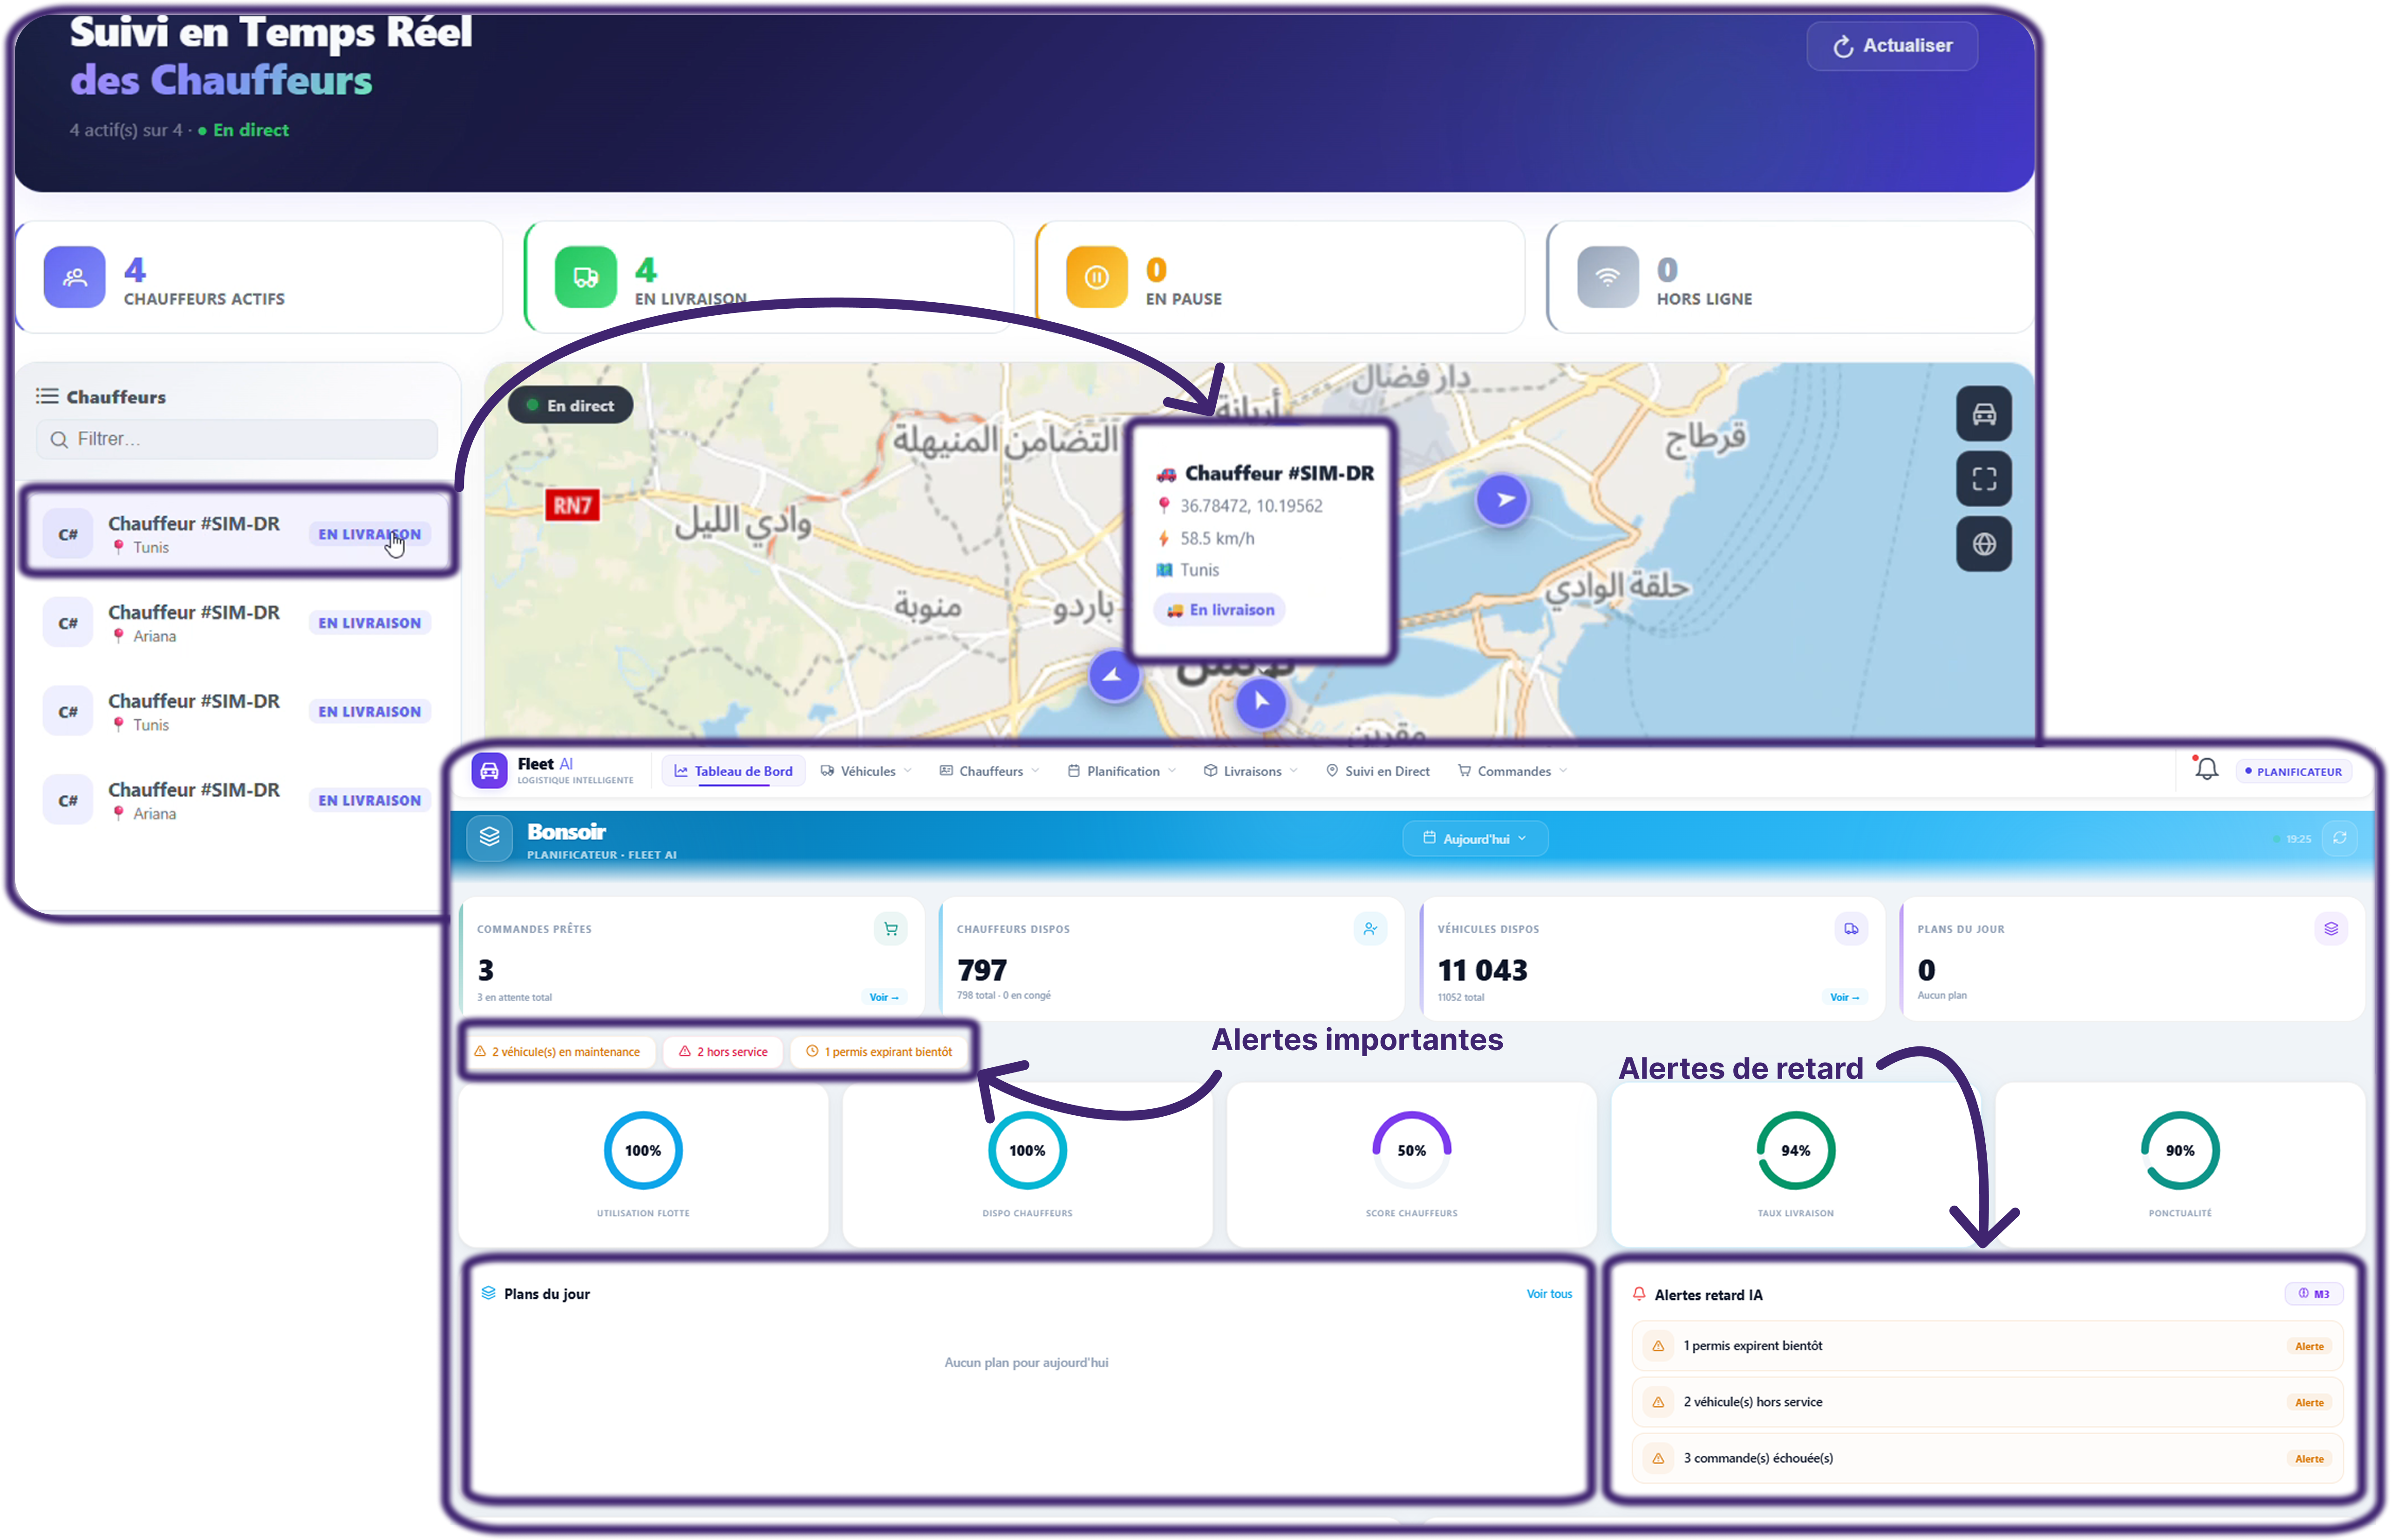
\includegraphics[width=\linewidth, keepaspectratio]{img/capture/web/sp4_tracking_kpi_composite}%
}{%
  \fbox{\parbox{0.9\linewidth}{\centering\vspace{4cm}\textit{[img/sp4\_tracking\_kpi\_composite]}\vspace{4cm}}}%
}
\caption{Carte GPS WebSocket, alertes retard et KPI journalier}
\label{fig:sp4-tracking}
\end{figure}

\subsection{Gestion des trois modes de paiement}

Le système prend en charge trois modes de paiement distincts, gérés exclusivement depuis l'interface web par le REC. Le mode \textbf{Prépayé} autorise la livraison automatiquement grâce au statut importé de l'ERP~: aucune action manuelle n'est requise. Le mode \textbf{Chèque} implique une capture OCR automatisée (GrepSys) par le Chauffeur, suivie d'une saisie dans PaySmart par le REC et d'une validation SMS envoyée au client. Le mode \textbf{Traite} requiert la photo de la traite et une décision explicite du REC (APPROUVÉ ou REFUSÉ avec motif obligatoire), tracée dans l'historique de paiement.

\begin{figure}[H]
\centering
\IfFileExists{img/capture/web/sp4_payment_composite.png}{%
  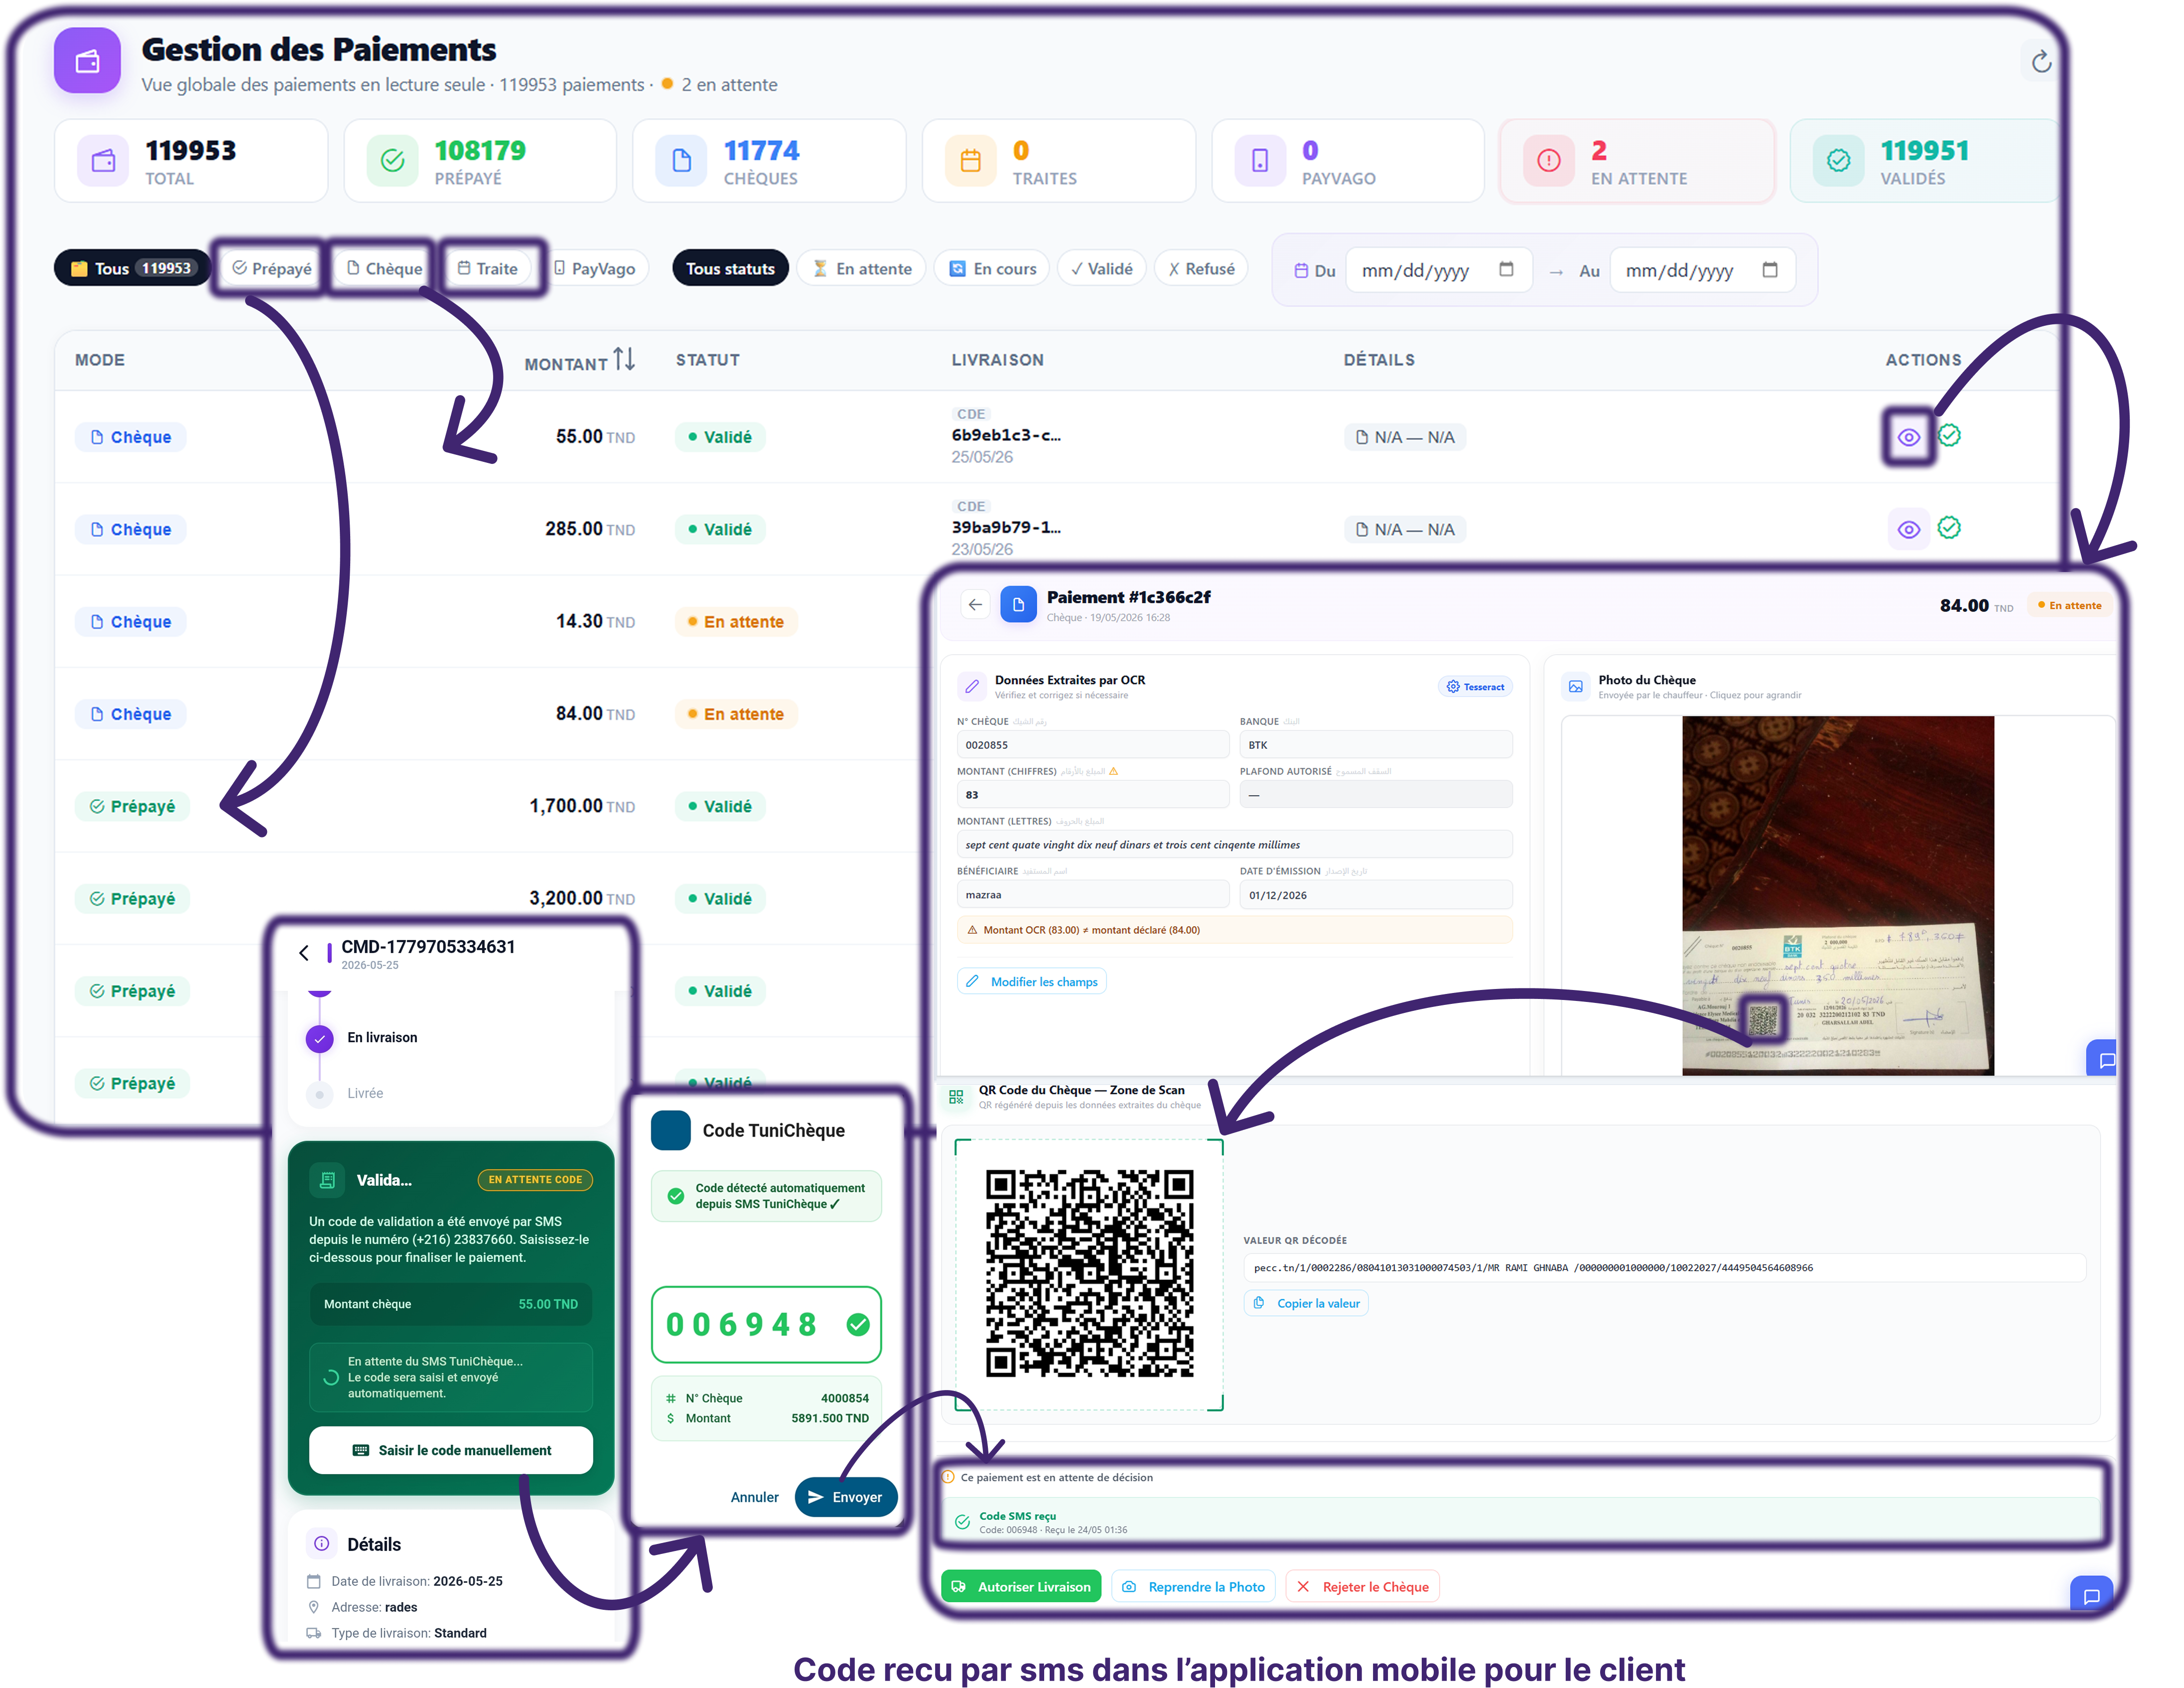
\includegraphics[width=\linewidth, keepaspectratio]{img/capture/web/sp4_payment_composite}%
}{%
  \fbox{\parbox{0.9\linewidth}{\centering\vspace{4cm}\textit{[img/sp4\_payment\_composite]}\vspace{4cm}}}%
}
\caption{Paiements : prépayé, chèque OCR et décision traite REC}
\label{fig:sp4-payments}
\end{figure}

\subsection{Gestion des livraisons échouées et reprogrammation}

En cas d'impossibilité de livrer, le Chauffeur signale le problème sur l'application mobile (CLIENT\_ABSENT, ACCES\_BLOQUE, REFUS\_CLIENT, MARCHANDISE\_ENDOMMAGEE, ADRESSE\_INCORRECTE). Le statut passe immédiatement à ÉCHOUÉE et une notification est envoyée au Planificateur et au REC. Depuis l'interface web, le Planificateur consulte la liste des livraisons échouées du jour et peut les reprogrammer en priorité le lendemain (J+1) avec réaffectation automatique.

\begin{figure}[H]
\centering
\IfFileExists{img/capture/web/sp4_reclamations_composite.png}{%
  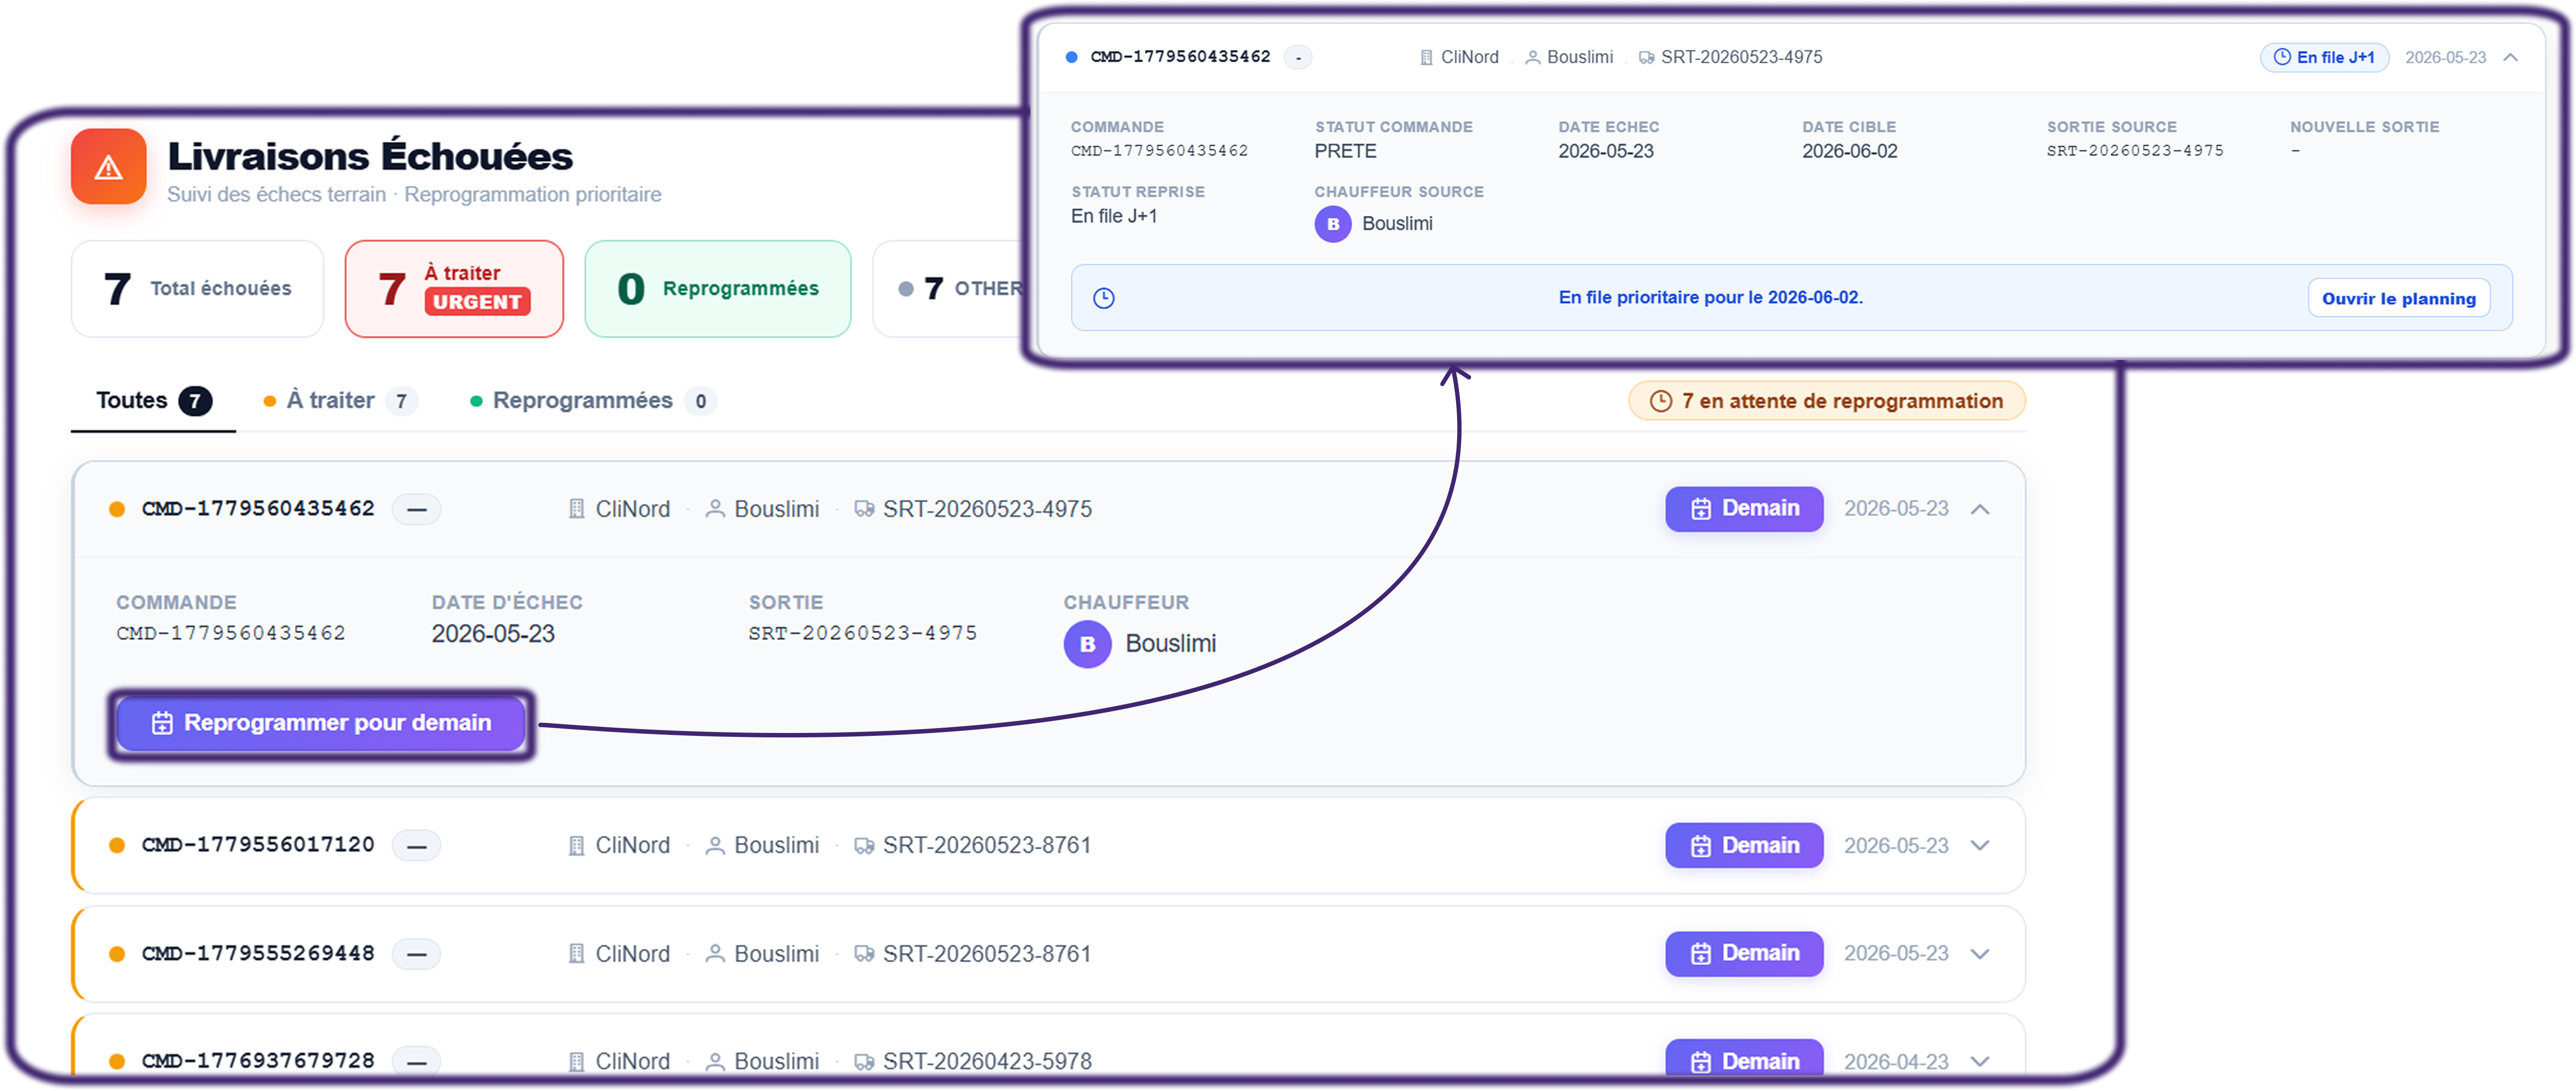
\includegraphics[width=\linewidth, keepaspectratio]{img/capture/web/sp4_reclamations_composite}%
}{%
  \fbox{\parbox{0.9\linewidth}{\centering\vspace{4cm}\textit{[img/sp4\_issues\_composite]}\vspace{4cm}}}%
}
\caption{Livraisons échouées : motifs et reprogrammation J+1}
\label{fig:sp4-issues}
\end{figure}

\subsection{Bordereaux de livraison et clôture de tournée}

En fin de journée, le REC génère depuis l'interface web un bordereau de livraison pour chaque tournée, récapitulant les montants encaissés par mode de paiement (espèces, chèque, traite) et le statut de chaque livraison (LIVRÉE / ÉCHOUÉE / REPORTÉE). Ce bordereau sert de document officiel de clôture de tournée. La réconciliation des encaissements par rapport aux commandes planifiées est effectuée automatiquement par le système.

\begin{figure}[H]
\centering
\IfFileExists{img/capture/web/sp4_recap_composite.png}{%
  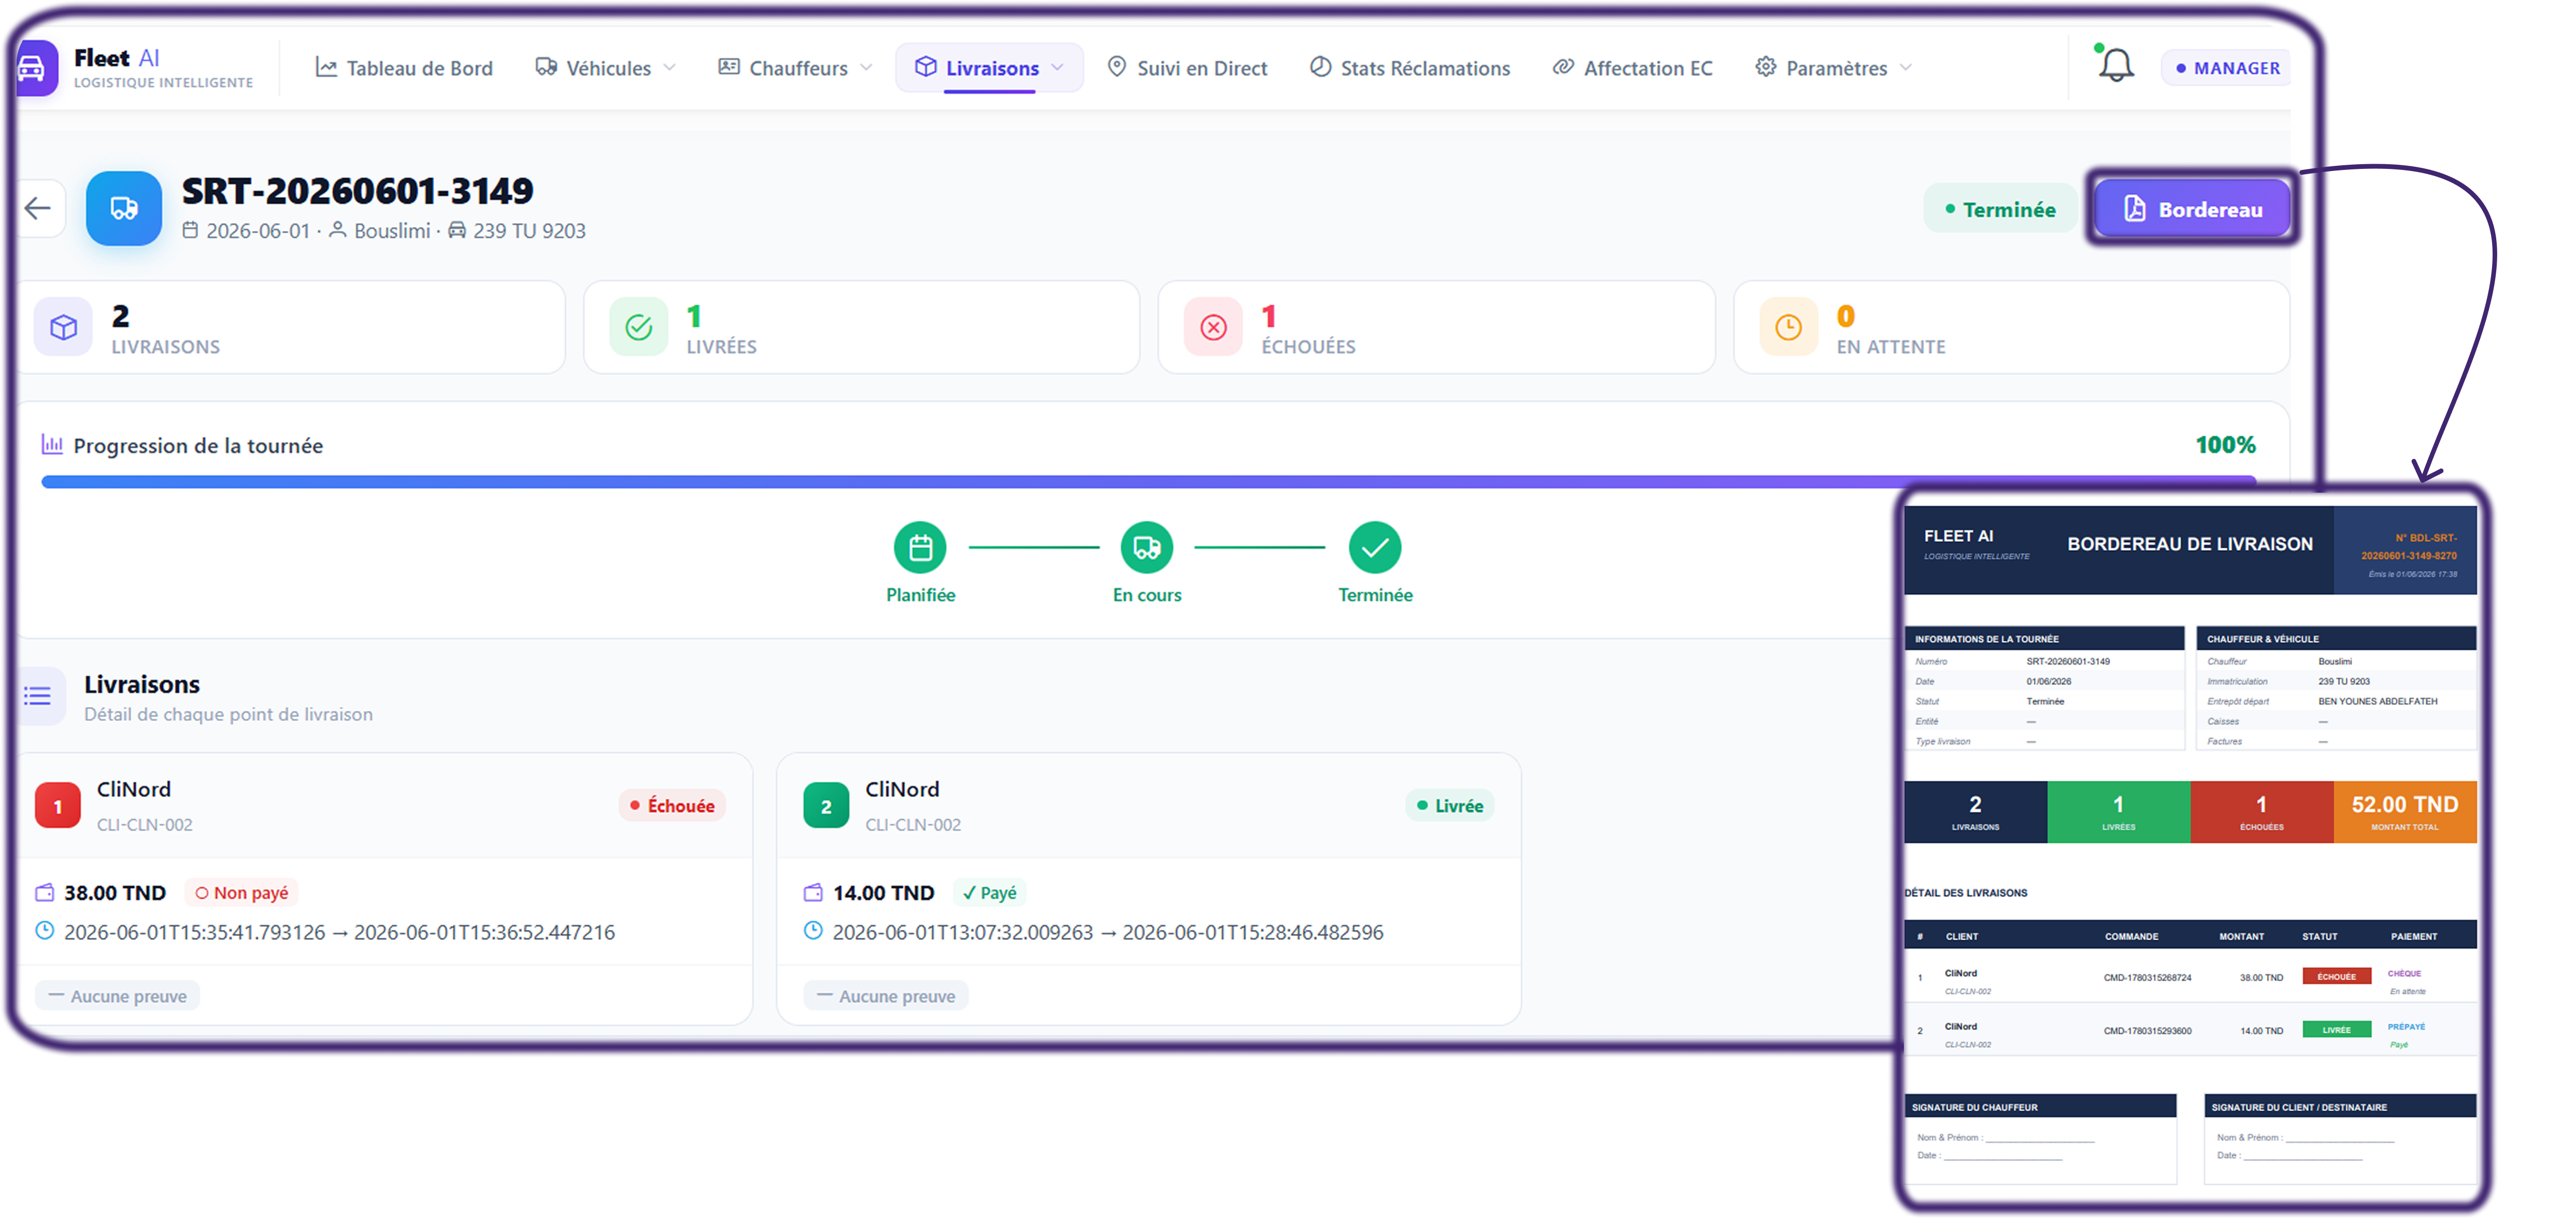
\includegraphics[width=\linewidth, keepaspectratio]{img/capture/web/sp4_recap_composite}%
}{%
  \fbox{\parbox{0.9\linewidth}{\centering\vspace{4cm}\textit{[img/capture/web/sp4\_recap\_composite.png]}\vspace{4cm}}}%
}
\caption{Bordereau de clôture et réconciliation encaissements}
\label{fig:sp4-recap}
\end{figure}

\subsection{Gestion et suivi des réclamations}

Le REC traite les réclamations clients depuis une interface web dédiée, avec visualisation du statut, du délai de traitement et de l'historique des échanges. Si une réclamation reste non traitée après 48~heures, le système l'escalade automatiquement au Manager avec notification. Depuis l'application mobile, le Client peut soumettre une réclamation en sélectionnant la catégorie et la description, et suivre l'état de traitement en temps réel de ses tickets ouverts (Ouvertes / En cours / Résolues).

\begin{figure}[H]
\centering
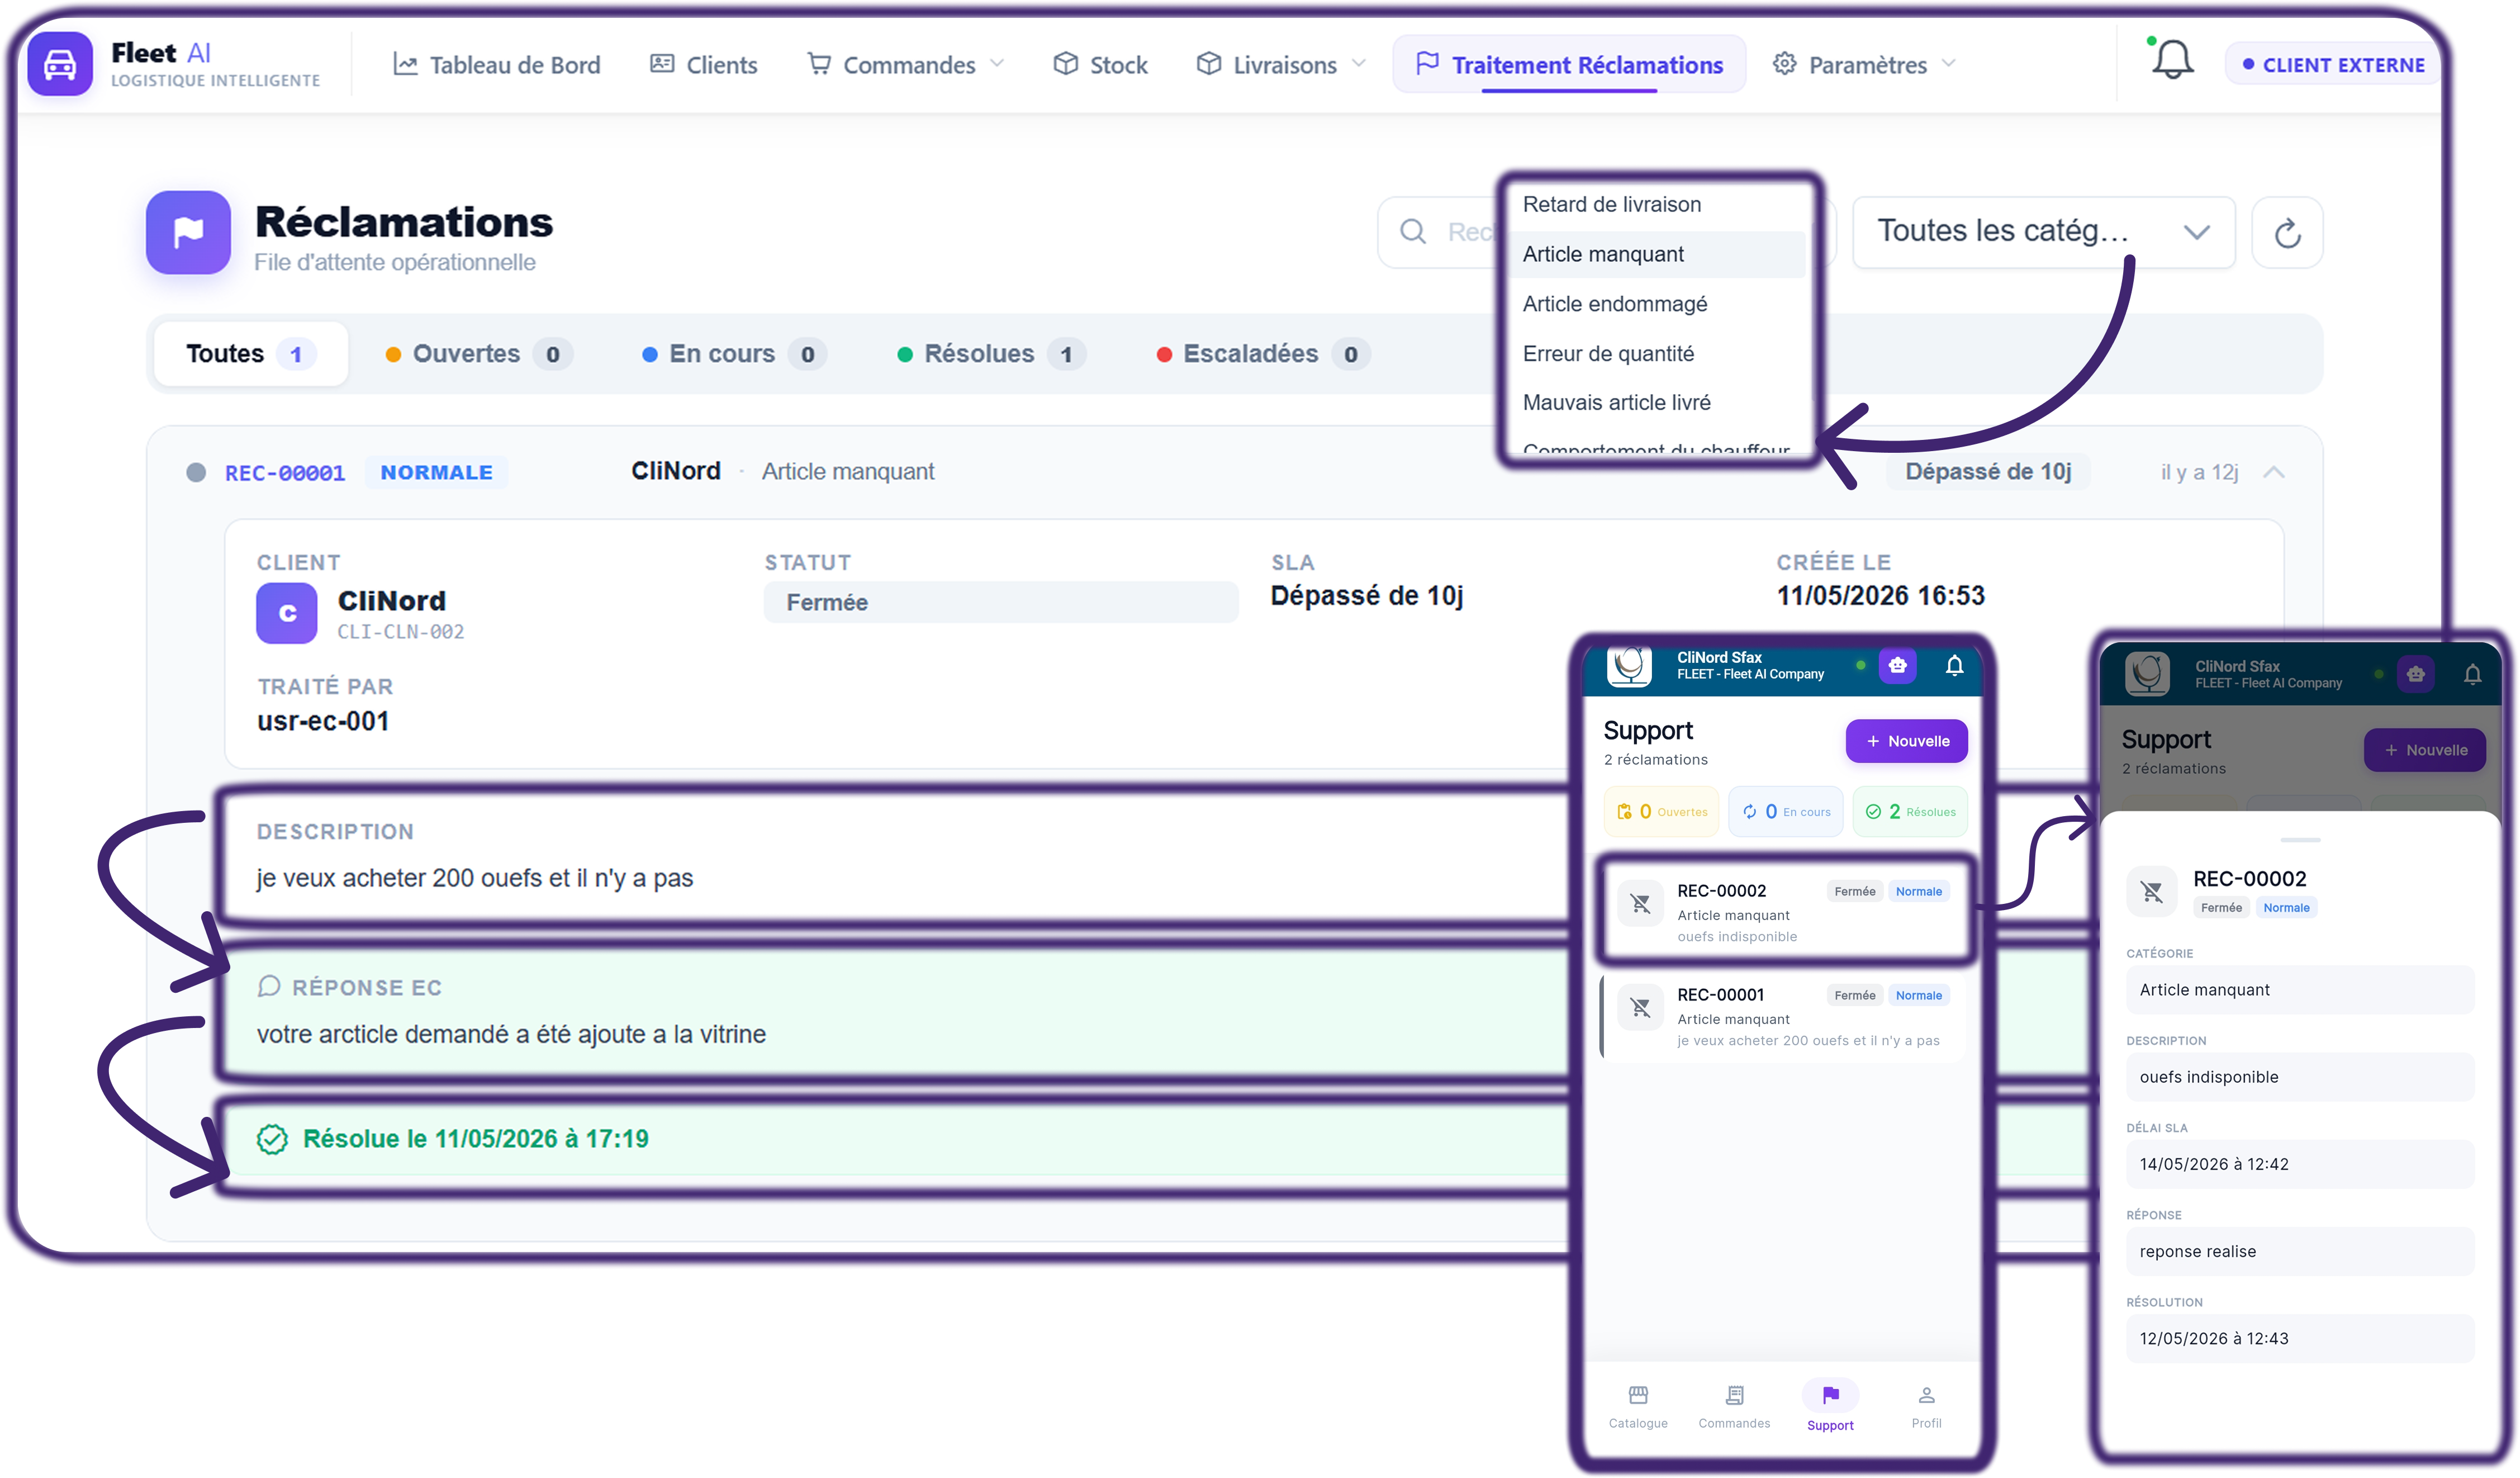
\includegraphics[width=\linewidth, keepaspectratio]{img/capture/mobile/support_client}
\caption{Interface Composite Web et Mobile --- Module Support : liste des réclamations avec statut et priorité (REC-00002, REC-00001), et détail d'un ticket avec catégorie, description, délai SLA, réponse du REC et date de résolution}
\label{fig:sp4-reclamations}
\end{figure}

\subsection{Application mobile Chauffeur --- Démarrage de sortie et checklist}

Avant sa première livraison, le Chauffeur accepte le plan qui lui a été attribué, valide la checklist de contrôle véhicule (niveau d'huile, carburant, rétroviseurs, documents, propreté, chargement sécurisé) puis autorise le suivi GPS en arrière-plan. Une fois la checklist validée, la sortie démarre : le statut passe à \textit{En cours}, la première livraison s'active automatiquement et l'itinéraire complet (578~km, 4 arrêts) est affiché sur la carte TomTom.

\begin{figure}[H]
\centering
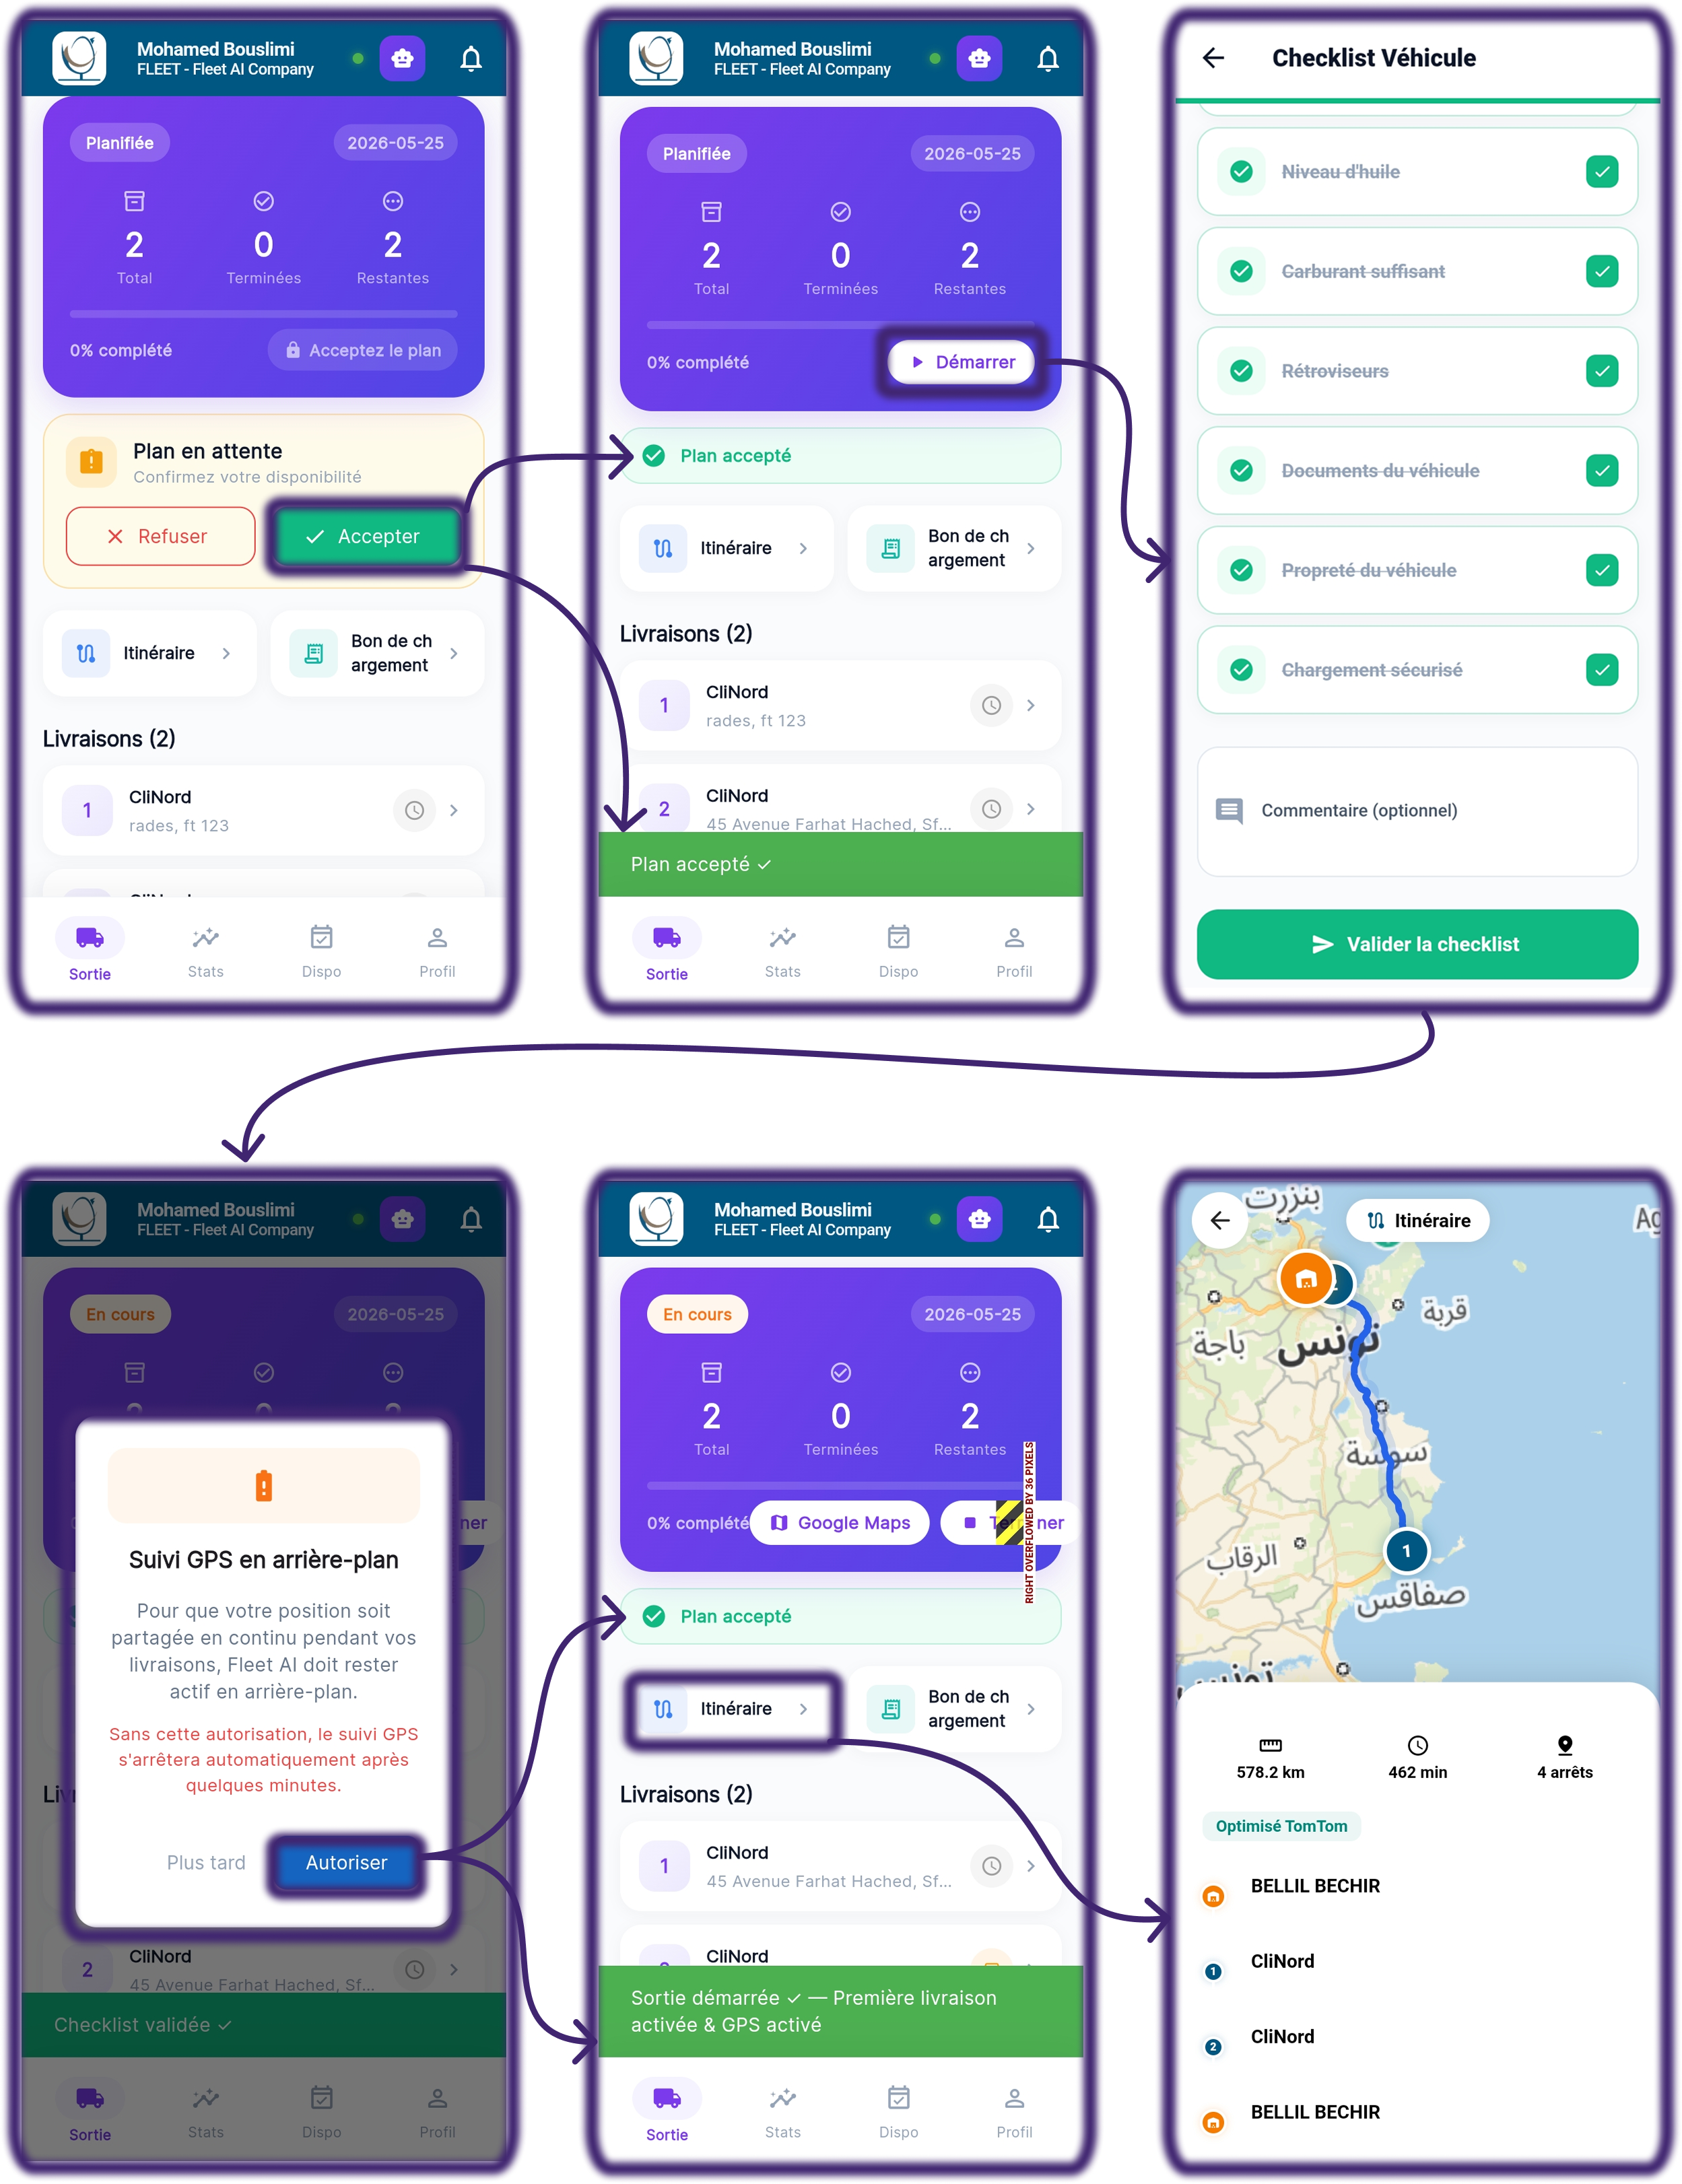
\includegraphics[width=\linewidth, keepaspectratio]{img/capture/mobile/debut_livraison_chauffeur}
\caption{Application mobile Chauffeur --- Démarrage de la sortie : (1)~plan en attente, acceptation, (2)~plan accepté avec bouton Démarrer, (3)~checklist véhicule complète, (4)~autorisation GPS arrière-plan, (5)~sortie démarrée avec activation livraison et (6)~itinéraire optimisé sur carte}
\label{fig:sp4-start}
\end{figure}

\subsection{Application mobile Chauffeur --- Finalisation et paiement de livraison}

A l'arrivée chez le client, le chauffeur signale son arrivée (ou elle est détectée automatiquement par le système GPS quand il entre dans le périmètre de l'adresse). Il consulte le bon de livraison PDF généré automatiquement, prend une photo de la marchandise remise, puis capture le paiement selon le mode indiqué (ici : chèque). L'écran de capture du chèque lui permet de photographier le titre et d'envoyer le montant au REC pour validation. La photo est transmise en temps réel et la livraison passe au statut LIVRÉE après confirmation.

\begin{figure}[H]
\centering
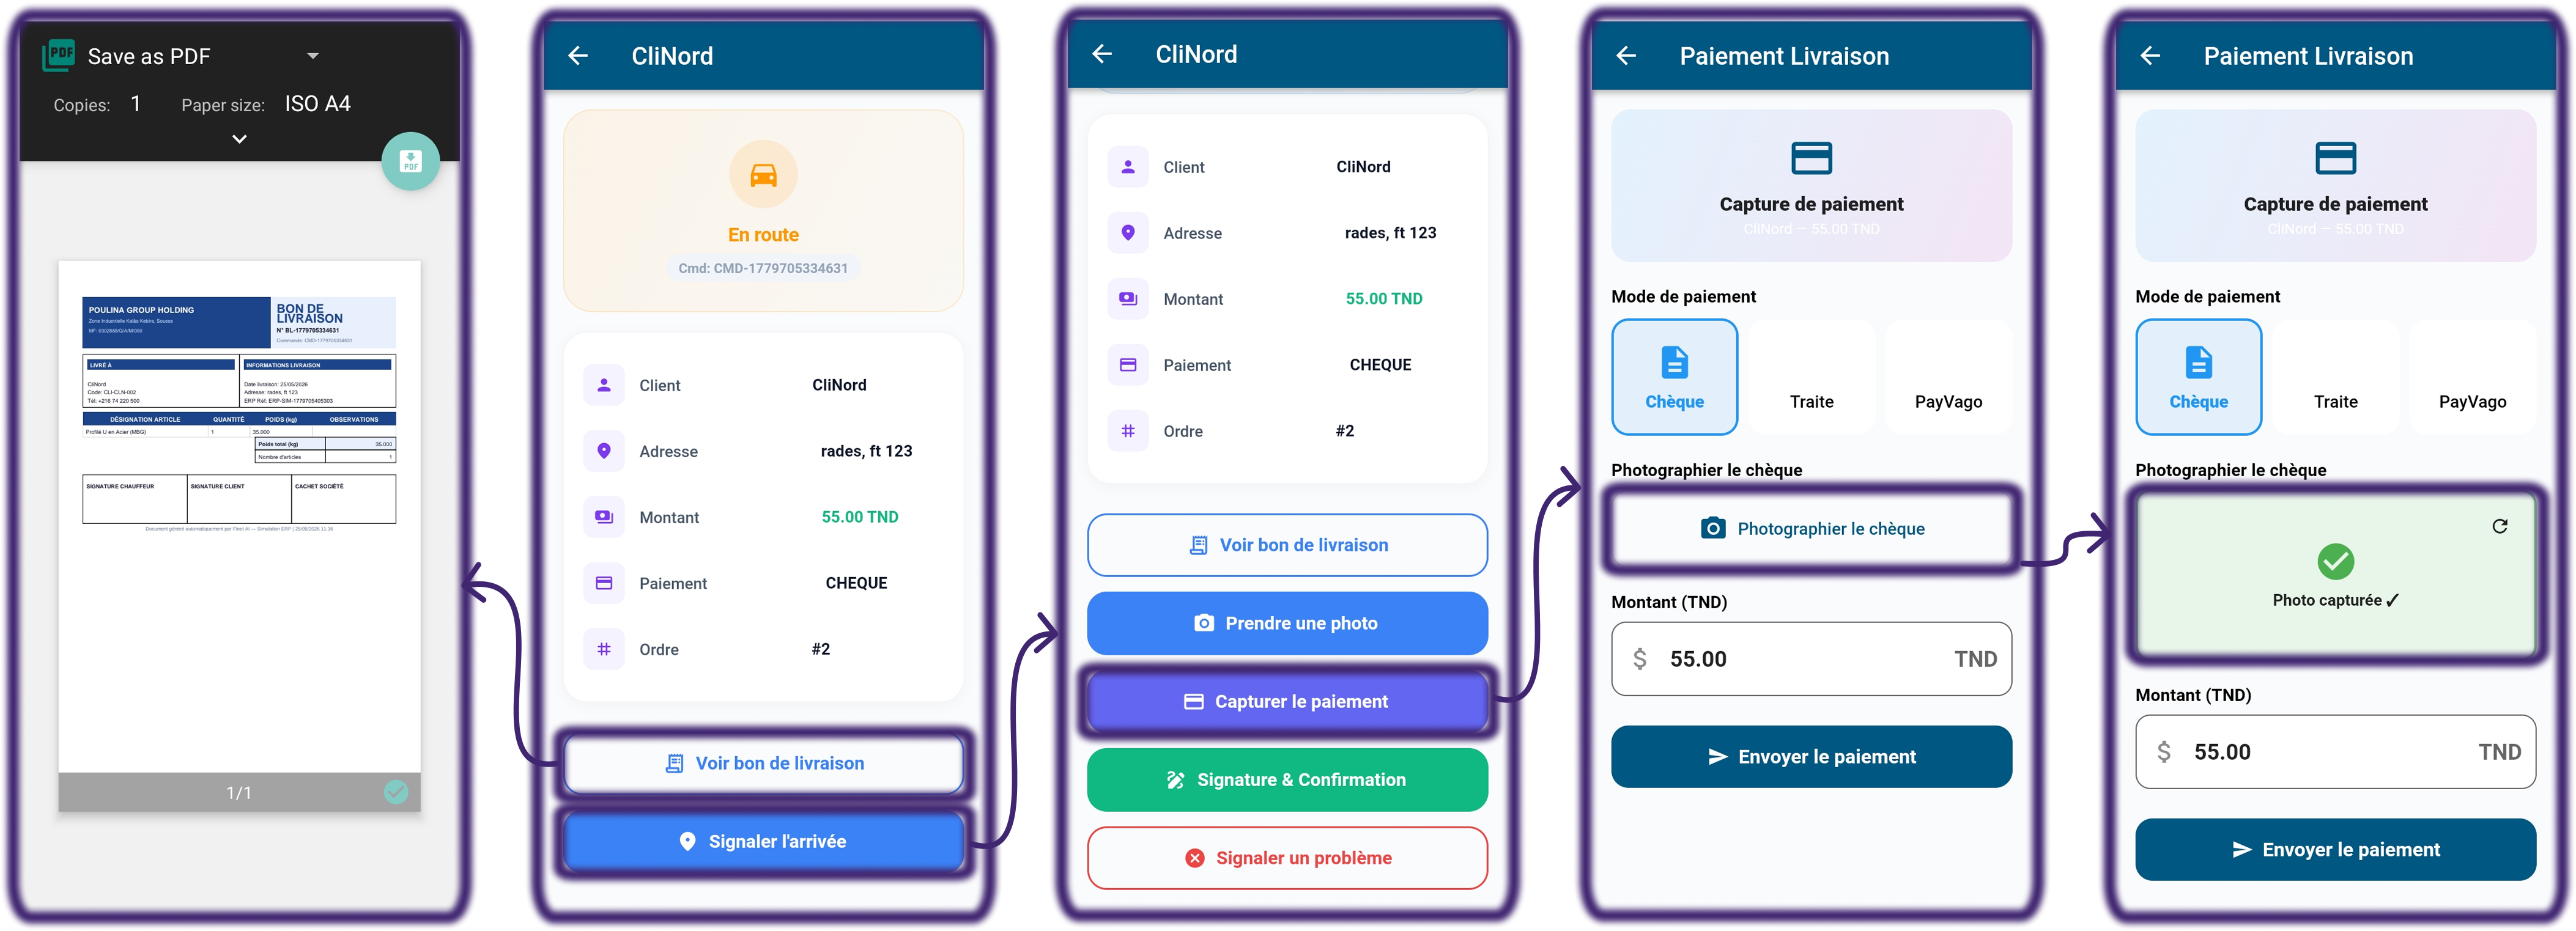
\includegraphics[width=\linewidth, keepaspectratio]{img/capture/mobile/finaliser_livraison_chauffeur}
\caption{Application mobile Chauffeur --- Finalisation de livraison : bon de livraison PDF, signalement d'arrivée, actions terrain (voir bon, prendre photo, capturer paiement, signature, signaler problème), capture du chèque avec photo et envoi au REC}
\label{fig:sp4-proof}
\end{figure}

% =============================================================
\section{Tests}
% =============================================================

\begin{figure}[H]
\centering
\IfFileExists{img/capture/web/sp4_test_browser.png}{%
  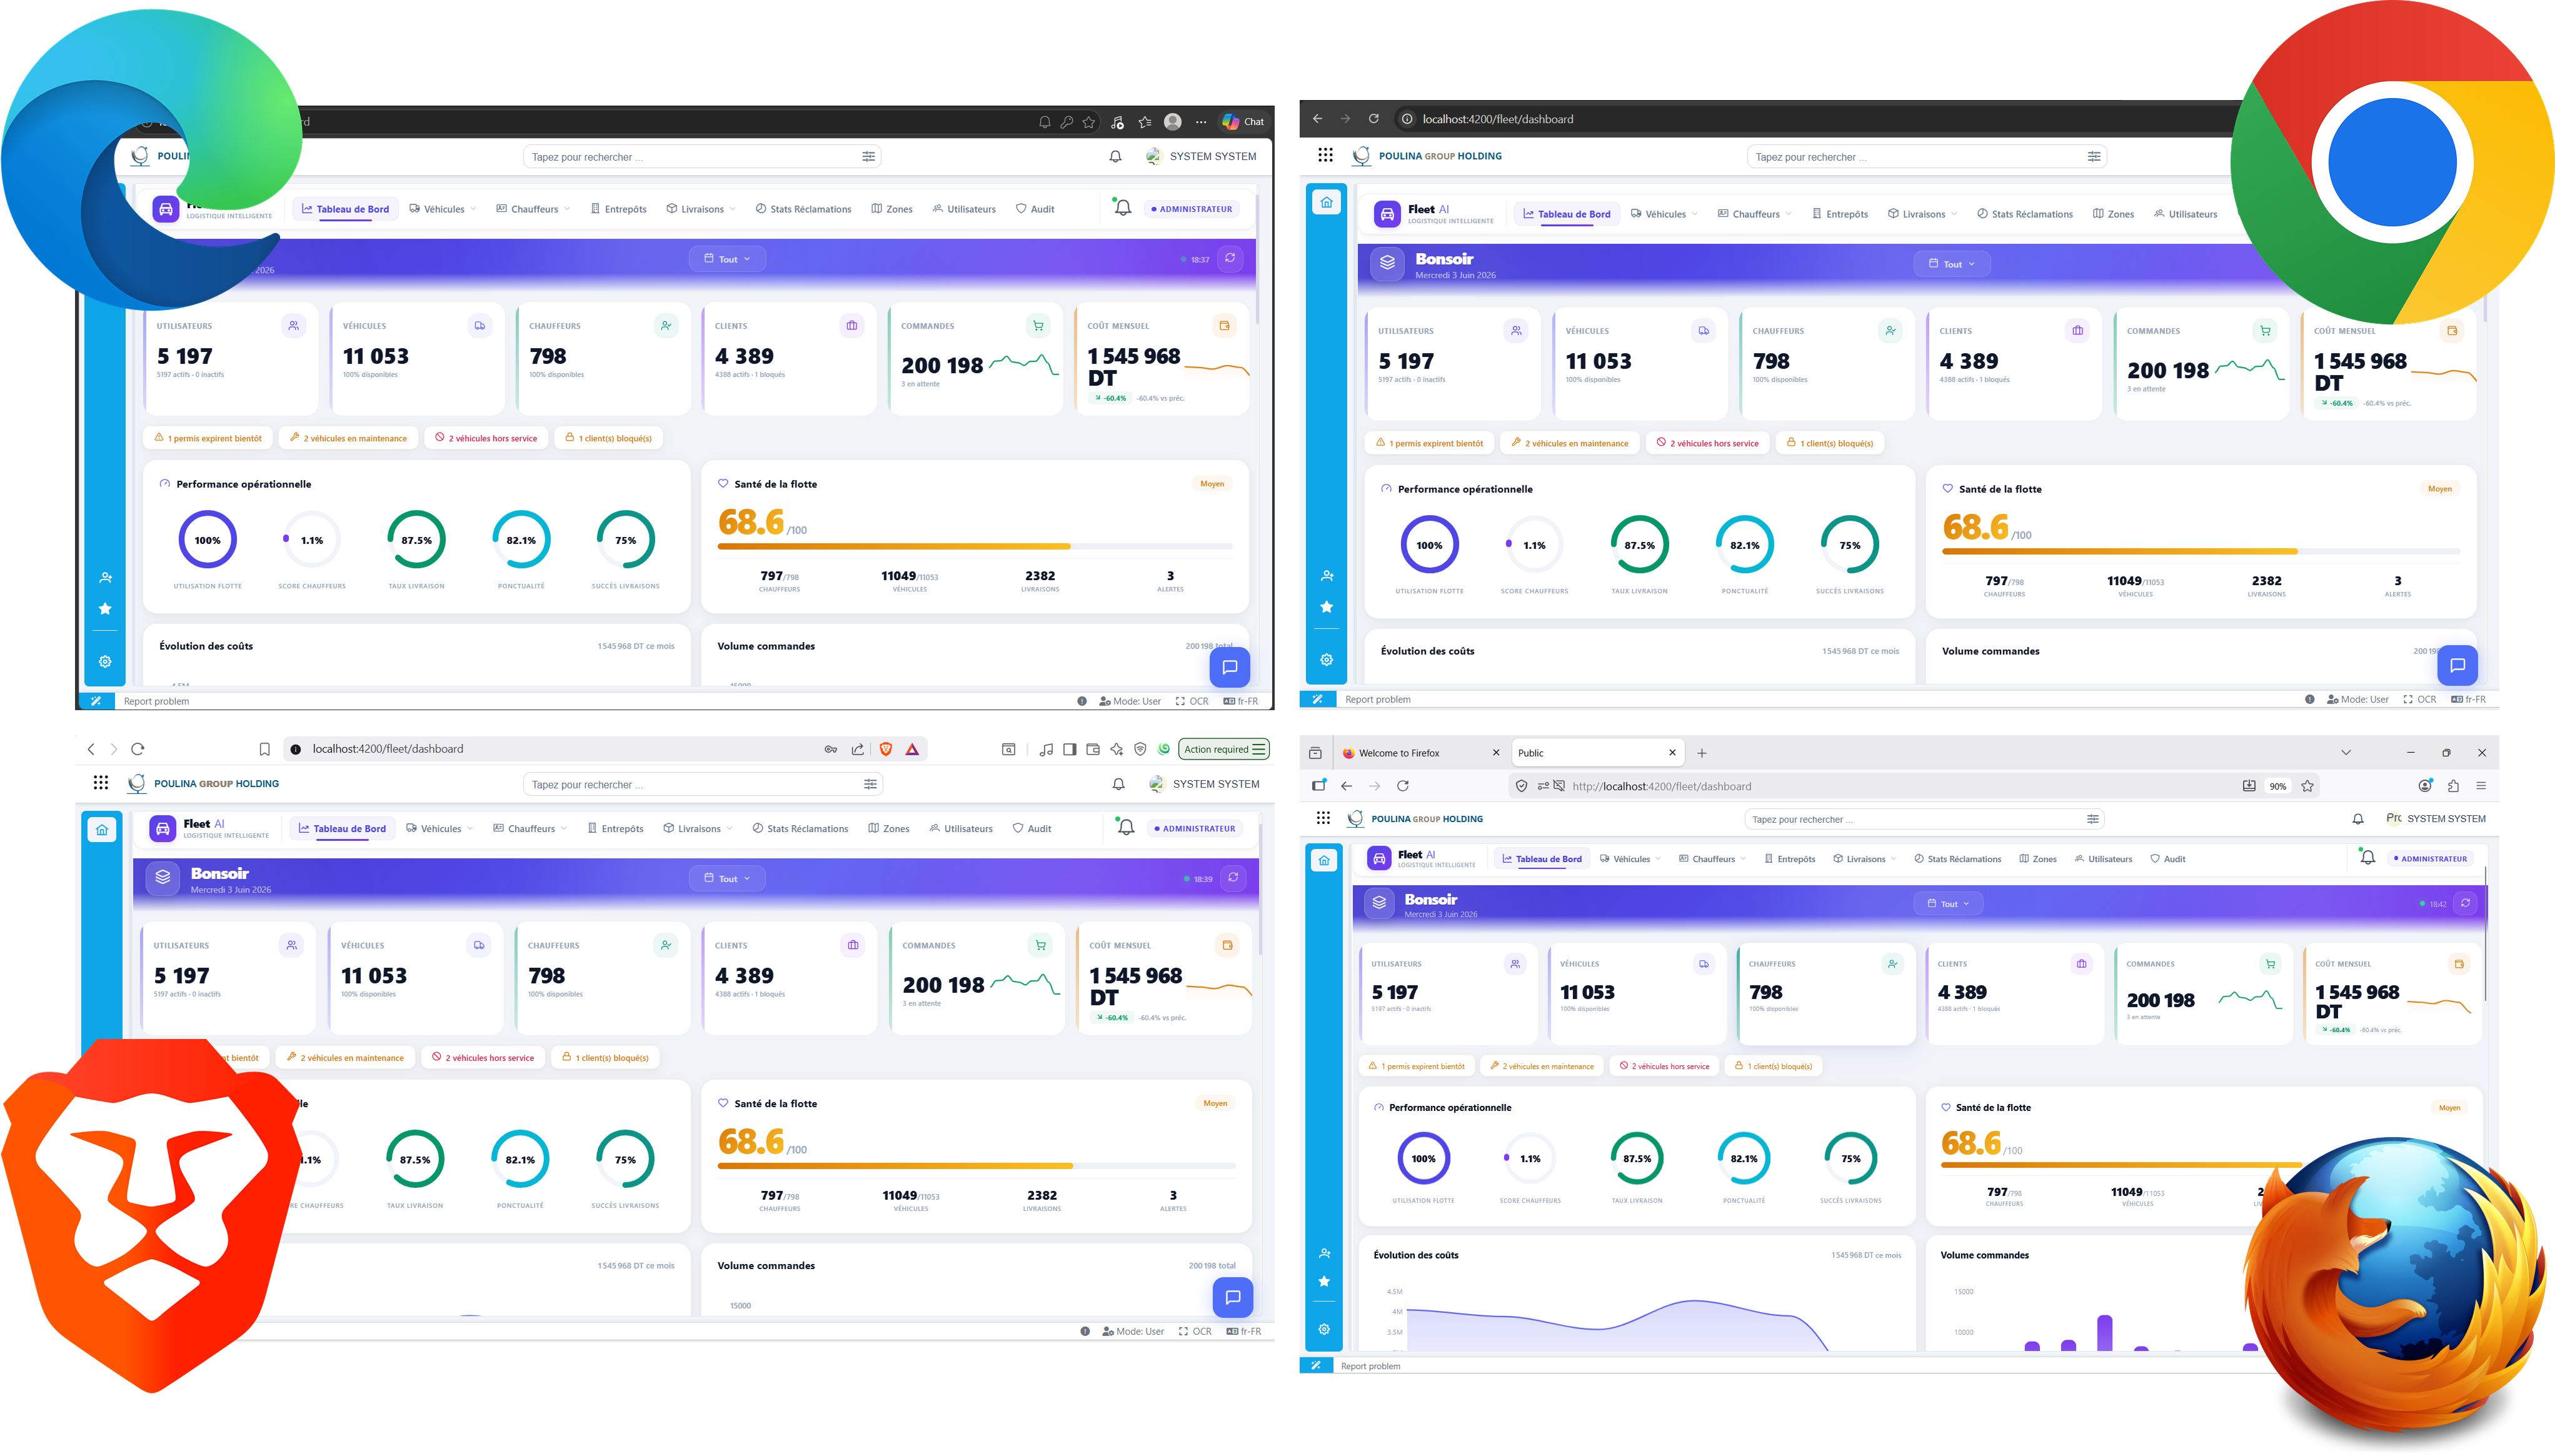
\includegraphics[width=\linewidth, keepaspectratio]{img/capture/web/sp4_test_browser}%
}{%
  \fbox{\parbox{0.9\linewidth}{\centering\vspace{4cm}\textit{[img/capture/web/sp4\_test\_browser.png]}\vspace{4cm}}}%
}
\caption{Exécution d'un test de navigateur sur la page de suivi GPS}
\label{fig:sp4-test}
\end{figure}

\section*{Conclusion}
\addcontentsline{toc}{section}{Conclusion}

Le Sprint~4 couvre l'intégralité de la phase d'exécution terrain de Fleet~AI : suivi GPS temps réel via WebSocket, gestion des trois modes de paiement, traitement des incidents et réclamations avec escalade automatique, et pilotage via tableaux de bord KPI journaliers. Les fonctionnalités de démarrage de sortie avec checklist véhicule, de confirmation terrain (prise de photo, capture chèque, signalement d'arrivée) et de support client sont illustrées par les captures de l'application mobile Flutter. Le Sprint~5 introduira la couche prédictive IA et l'assistant conversationnel.
